% This is the root file of your thesis: thesis.tex
% A line starting with % is a comment. In some cases, I have included a command preceded by a %. You may activate the command by removing the %.

%%===================================
\documentclass[12pt, twoside, openright]{report}
\usepackage{ramsstyle}
\usepackage{float}
\usepackage{hyperref}
\usepackage{longtable}
\usepackage{subfigure}
\usepackage{tabularx}
\newcolumntype{C}[1]{>{\centering\arraybackslash}p{#1}}
\usepackage{pdfpages}
\usepackage{wrapfig}
\usepackage{tocbibind}
\usepackage[bottom]{footmisc}
%%===================================
%Write the various parts of your thesis as separate files and include them into the main file by the command \include{name of included file}. When you compile the LaTeX file, you may choose which subfiles to include by the command
%%===================================
\begin{document}
%\setcounter{page}{0}
%This is the Titlepage
%%=========================================
\thispagestyle{empty}
\includegraphics[scale=0.8]{fig/NTNU}
\mbox{}\\[2pc]
\begin{center}
\Huge{Drop and Recovery of Sensor Nodes Using UAVs}\\[3pc]

\Large{Vegard Voldsund}\\[1pc]
\large{June 2014}\\[4pc]

MASTER THESIS\\
Department of Engineering Cybernetics\\
Centre for Autonomous Marine Operations and Systems\\
Norwegian University of Science and Technology
\end{center}
%\begin{figure}[H]
%\center
%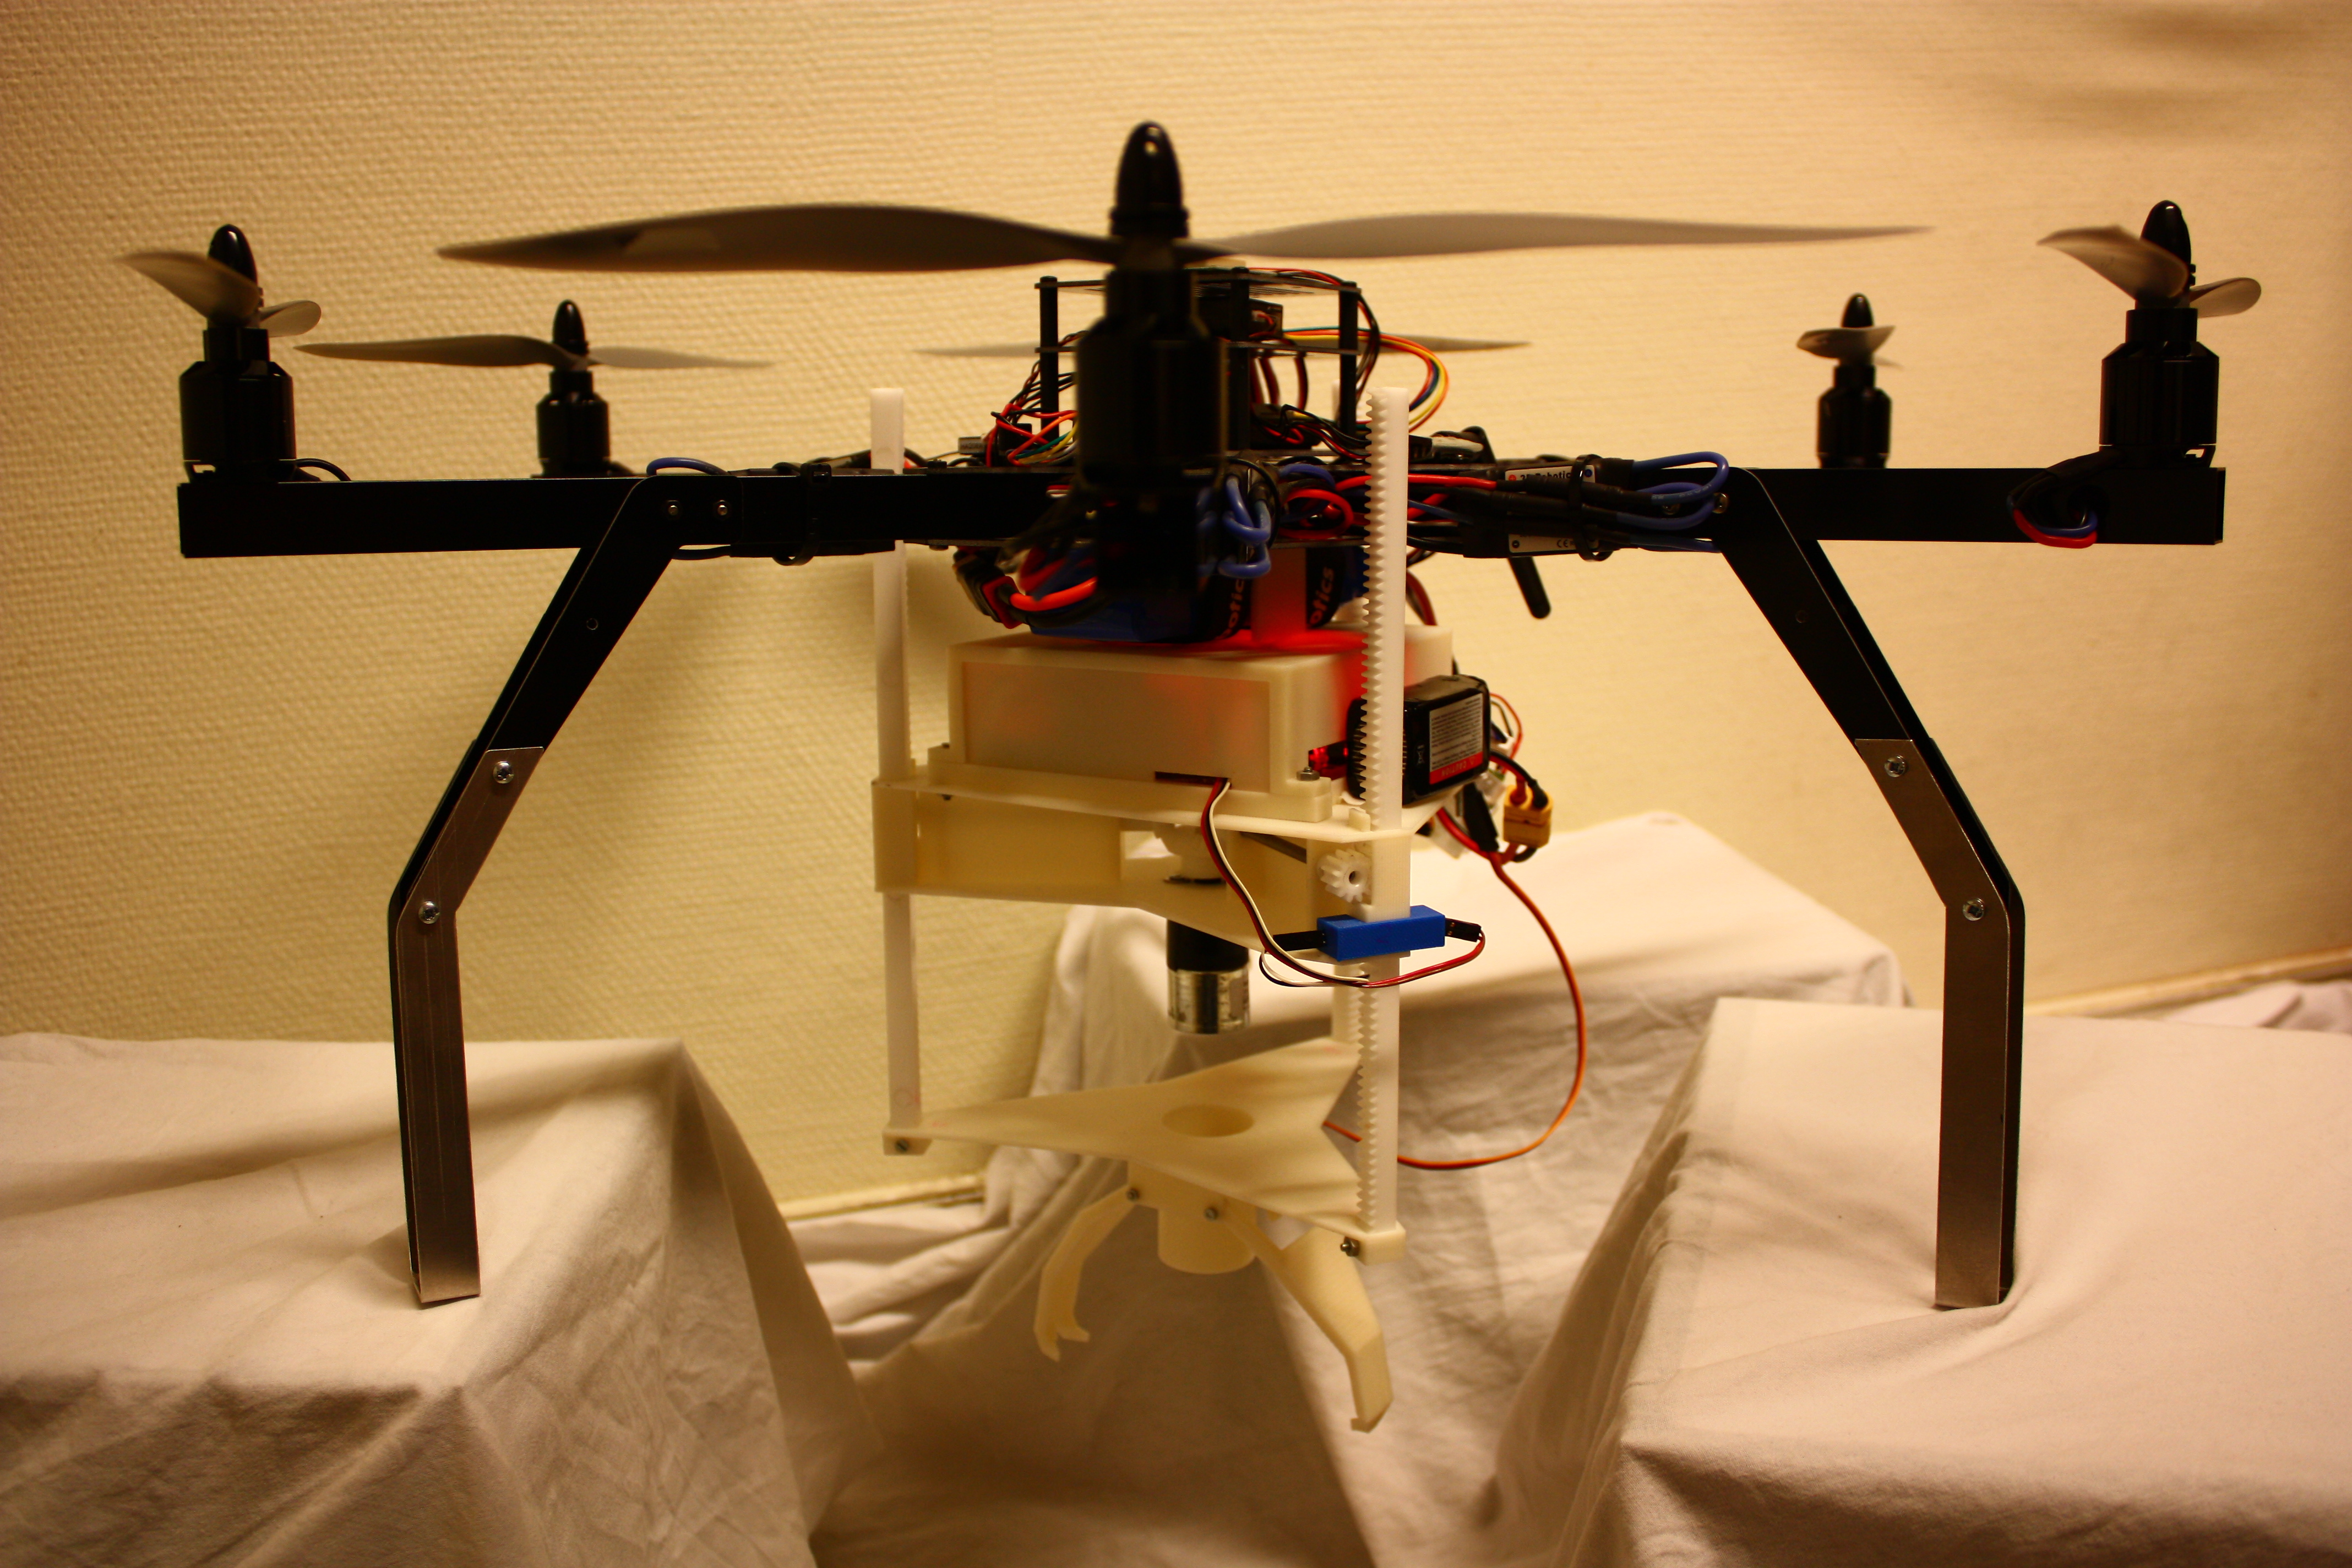
\includegraphics[width=10 cm]{fig/finished/finished.jpg}
%\end{figure}
\vfill

\noindent Supervisor 1: Professor Tor Arne Johansen 

\noindent Supervisor 2: PhD Candidate Kristian Klausen

 % This is the titlepage
\pagenumbering{roman}
\setcounter{page}{0}
%\chapter*{Problem Description}
%\includegraphics[scale=0.6]{oppgave.pdf}
\addcontentsline{toc}{chapter}{Problem Description}
\vspace*{\fill}
\includepdf[offset = 0cm -5cm, scale = 1, pages=1, pagecommand=\chapter*{Problem Description}]{oppgave.pdf}



\include{abstract}
%This is the Summary
%%=========================================
\addcontentsline{toc}{chapter}{Sammendrag}
\chapter*{Sammendrag}
\textit{(Norwegian translation of the abstract)}\\
\newline

%This is the Preface
%%=========================================
\addcontentsline{toc}{chapter}{Preface}
\chapter*{Preface}
This project is written as a part of my MSc degree at the Department of Engineering Cybernetics at NTNU  and is part of research conducted by the Center of Autonomous Marine Operations and Systems (AMOS). The work in this project will be continued into my master thesis.\\
\newline
The execution of this project would not have been possible without the financial backing from AMOS and the usage of equipment at the electronics and mechanical workshops at the Department of Engineering Cybernetics, NTNU. I will like to thank the guys at these workshops for valuable help and guidance.\\
\newline
I would also like to thank my supervisors Professor Tor Arne Johansen and PhD Candidate Kristian Klausen for guidance and encouragement along the way.\\
\newline
\begin{flushright}
\textit{Vegard Voldsund}
\end{flushright}
%This is Appendix A - Acronyms
%%=========================================
\addcontentsline{toc}{chapter}{Acronyms}
\chapter*{Acronyms}
\begin{tabular}{l l}
\textbf{AMOS} & Centre for Autonomous Marine Operations and Systems\\
%\textbf{APM 2.6} & Ardupilot Mega 2.6\\
%\textbf{BGR} & Blue-Green-Red\\
%\textbf{CEP} & Circular Error Probability\\
%\textbf{CPU} & Central Processing Unit\\
%\textbf{DH Convention} & Denavit-Hartenberg Convention\\
%\textbf{ECEF} & Earth-centered Earth-fixed\\
%\textbf{GPS} & Global Positioning System\\
%\textbf{HSV} & Hue-Saturation-Value\\
%\textbf{IC} & Integrated Circuit\\
%\textbf{IMU} & Inertial Measurement Unit\\
%\textbf{I/O} & Input/Output\\
%\textbf{IR} & Infrared Radiation\\
%\textbf{ISA} & Inertial Sensor Assembly\\
%\textbf{LBP} & Local Binary Patterns\\
%\textbf{LED} & Light Emitting Diode\\
%\textbf{MAVLink} & Micr Air Vehicle Protocol\\
%\textbf{MEMS} & Microelectromechanical Systems\\
%\textbf{MIPI} & Mobile Industry Processor Interface\\
%\textbf{NED} & North-East-Down\\
%\textbf{OpenCV} & Open Source Computer Vision Library\\
%\textbf{PWM} & Pulse-Width Modulation\\
%\textbf{RAM} & Random Access Memory\\
%\textbf{SIFT} & Scale-Invariant Feature Transform\\
%\textbf{SURF} & Speeded-Up Robust Features\\
%\textbf{UART} & Universal Asynchronous Receiver/Transmitter\\
%\textbf{UAV} & Unmanned Aerial Vehicle\\
%\textbf{WGS-84} & World Geodetic System 84\\
\end{tabular}

%\addcontentsline{toc}{chapter}{Contents}
\tableofcontents
%\addcontentsline{toc}{chapter}{List of Figures}
\listoffigures
\listoftables
%\addcontentsline{toc}{chapter}{List of Tables}
\pagenumbering{arabic}
\setcounter{page}{0}
%This is chapter 1
%%=========================================
\chapter{Introduction}
%%=========================================
\section{Background and motivation}
Unmanned aerial vehicles (UAVs) are aircraft without a human operator on board. They can fly autonomously or be remotely operated by a pilot on the ground. The use of UAVs have exploded in recent years. This is due to a lot of ongoing research and development conducted by companies, scientists and enthusiasts. Some of this research and development have resulted in open source projects that have made advanced UAV technology availably at very low cost.\\
\newline
The UAV used in this project will be based on one of these open source UAV solutions. This solution is chosen because it is cost efficient, results of the project will be easy to use by others, and it is a way to get going fast and still be able to do some customization.\\
\newline
This project is a part of research conducted by the Center of Autonomous Marine Operations and Systems (AMOS) at NTNU. AMOS is now establishing a new laboratory with field experimental capabilities (UAV-Lab). This project is related to this lab. To be a part of the research at AMOS opens up a lot of opportunities, but it also means that some things have to be standardized. For instance the choice of UAV and the use of PandaBoard as onboard computer follows standards decided by AMOS. Use of DUNE as an environment to structure and develop the software running on the onboard computer and the use of NEPTUS as a ground control station is also according to AMOS standards.\\
\newline
The goal of this project is to create a mechanism that can be used for sensor node pickup and deployment by the use of multicopters. The sensor node will be a lightweight packet that can contain different sensors depending on the mission. These sensor nodes will be dropped into the sea where they will float on the surface. Examples of use for the sensor nodes can be to log temperature, currents, salinity or water quality. Hence they can be very useful in for instance climate research or for detecting oil spills.\\
\newline
Both fixed-wing and multicopter UAVs will be part of the sensor node pickup and deployment system and supplement each other in the UAV-lab. Multicopters will be used in coastal areas and at relatively good weather conditions, while fixed-wing UAVs have a much greater range and will be used for longer missions and in rougher weather conditions.\\
\newline
The project will be continued into a master thesis where the created mechanism will be used for sensor node pickup and deployment. This means that the goal of this project is not to create a fully operational system with seamless integration between the modules, but to make different modules that are ready to be used in the master thesis. This report should be read in this context.
\section{Previous work}
As already mentioned there has been a lot of research on UAVs in recent years, but most of this research have focused on fixed-wing aerial vehicles. And the applications have usually been limited to monitoring and search \citep{Mellinger2011}.\\
\newline
The latest couple of years have shown some research on rotary-wing aircraft interacting with the environment in different ways. There have been conducted research where the UAV is used to manipulate its environment. Two examples of this using two different strategies are \citep{jiang} and \citep{cartesian}. Lippiello and Ruggiero are inspired by the use of impedance control in robot manipulation tasks, while Jiang and Voyles alters a hexacopter by tilting the motors, making it possible to create a horizontal force without tilting the hexacopter.\\ 
\newline
The most relevant applications to highlight in this report are those that use different strategies for drop off and pickup of objects. Possibilities of using an avian catching fish as an inspiration for a quadcopter based gripper system to be able to execute high speed pickup have been explored by \citep{Thomas2013}. A gripper on the end of a link with two joints is used to replicate an avians leg and claw. Good results were achieved as the quadcopter was able to grasp targets at speeds up to 3 m/s. The trajectory of the pickup was decided pre run time to match the trajectory of the avian. Feedback to the controller was given using VICON\footnote{A very accurate external motion capture system}.\\
\newline
The use of a helicopter to grasp objects on the ground are explored in \citep{Pounds}. The ability to grasp objects of different shapes and without a perfect lined up position is in focus for the gripper design. Tests demonstrated an ability to grasp objects of different shapes and sizes under human control of the helicopter. The most difficult objects were grasped 67 \% of the time, while the easiest object was grasped 100 \% of the time.\\
\newline
Estimation of payload parameters are explored in \citep{Mellinger2011} as well as mechanical design and controller for aerial grasping. Relevant parameters to estimate are mass and inertia. These estimates can be used to adapt the controller and to check if the object was successfully picked up or not.
\section{Contribution and scope of this report}
Some of the research presented in the previous section picks up objects lying on the ground (in some of them at exactly known positions). The fact that the aim in the master project is to pick up sensor nodes that are floating affected by waves, wind and currents add another dimension to the challenge. Navigation at sea means that one can not rely on external sensor systems like for instance VICO. This means that accurate positioning above the sensor node will be a challenge. The UAV will have to rely on poor position measurements and some added sensor system, for instance camera, to close the loop between the UAV and the sensor node.\\
\newline
This project aims to connect known techniques and theory from different fields in new ways to make pickup and deployment of sensor nodes by the use of UAVs at sea possible.
\section{Organization of this report}
The UAV used in this project is described in Chapter 2. This description includes the most relevant features to give the reader insight into which possibilities that lie within the UAV. The PandaBoard that is used as onboard computer is also described for the same reasons.\\
\newline
Different possible design solutions are described in Chapter 3. The chapter starts with some design choices that are common for all the solutions and continues with specifics about the different proposals. Both advantages and limitations of the different solutions are considered before the chapter ends in a conclusion of which design solution to implement.\\
\newline
An introduction to the relevant reference frames used for navigation, control and object tracking, as well as some features of the open source computer vision library OpenCV are given in Chapter 4.\\
\newline
Chapter 5 presents the implementation of the chosen design solution. It covers mechanical design, node tracking using camera, communication between the different modules, some circuit design and power supply.\\
\newline
The tests of the design solution with associated results are described in Chapter 6. Some of the key features that are tested are weight limitations on the sensor node, accuracy of the node tracking  and robustness of the mechanical design.\\
\newline
The implemented design solution is discussed in Chapter 8, before conclusions are drawn in Chapter 9.\\
\newline
The digital appendix included with this report contains source code used for the experiments and the node tracking algorithm. Solidworks models of the 3D-printed parts are included as a resource if the reader wants to replicate the design solution.
\chapter{Background Theory}
\section{Reference Frames}
The main reference frames that are relevant for navigation and control are ECEF, NED and BODY. A brief introduction to these reference frames based on \citep{Fossen} and \citep{vik} follows. Denavit-Hartenberg convention (DH convention) is a useful tool for defining reference frames. A brief introduction to DH convention based on \citep{Spong} follows.
\subsubsection{ECEF}
The Earth-centered Earth-fixed (ECEF) reference frame has its origin fixed to the center of the earth while rotating with the earth. The x-axis is defined to point at the intersection between the $0^{\circ}$ longitude and the $0^{\circ}$ latitude. The z-axis points along the earths rotation axis and the y-axis complete the right handed orthogonal coordinate system.\\\newline
The position in the ECEF frame can be expressed both with Cartesian coordinates ($x_e$, $y_e$, $z_e$) and with ellipsoidal coordinates (longitude ($l$), latitude ($\mu$), height ($h$)). The transformation from Cartesian ECEF-coordinates to ellipsoidal ECEF-coordinates is given by
\begin{eqnarray}
\begin{bmatrix}
x_e\\
y_e\\
z_e
\end{bmatrix}  = \begin{bmatrix}
(N + h)\cos \mu \cos l\\
(N + h)\cos \mu \sin l\\
(\dfrac{r_p^2}{r_e^2}N + h) \sin \mu
\end{bmatrix}
\end{eqnarray}
where $r_e$ = 6378137 m is the equatorial radius of ellipsoid and $r_p$ = 6356752 m is the polar axis radius of the ellipsoid as defined in WGS-84. The parameter $N$ is the radius of curvature in prime vectorial obtained from \citep{vik}. 
\begin{eqnarray}
N = \dfrac{r_e^2}{\sqrt{r_e^2 \cos ^2 \mu + r_p^2 \sin ^2 \mu}}
\end{eqnarray}
The transformation from Cartesian coordinates to ellipsoid coordinates is a bit more complicated. Longitude is calculated straight forward as
\begin{eqnarray}
l = \tan ^{-1} (\dfrac{y_e}{x_e})
\end{eqnarray}
but the calculations of latitude  and height are implicit equations
\begin{eqnarray}
\tan(\mu) &=& \dfrac{z}{p}(1 - e^2\dfrac{N}{N + h})^{-1}\\
h &=& \dfrac{p}{\cos(\mu)} - N
\end{eqnarray}
where $e$ is the eccentricity of the Earth given by
\begin{eqnarray}
e = \sqrt{1 - (\dfrac{r_p}{r_e})^2}
\end{eqnarray}
There are several algorithms that can be used to solve these implicit equations, see for instance Algorithm 2.4 in \citep{Fossen}.
\subsubsection{NED}
The north-east-down (NED) reference frame is moving with the body. The x-axis is always pointing north, the y-axis is pointing east and the z-axis i pointing down normal to the Earth surface.
\subsubsection{BODY}
The BODY reference frame is body fixed and rotates and moves with the body. It is usually defined with the x-axis pointing along the longitudinal axis, the y-axis pointing along the transversal axis and the z-axis pointing along the normal axis of the body.
\subsubsection{Transformation Between ECEF and NED}
A vector defined in NED can be transformed to the ECEF frame by the use of a rotation matrix that defines the relationship between NED and ECEF reference frames.
\begin{eqnarray}
\boldsymbol{p}^e = \boldsymbol{R}_n^e(\boldsymbol{\Theta} _{en})\boldsymbol{p}^n\\
\boldsymbol{\Theta} _{en} = \begin{bmatrix}
l & \mu & h\\
\end{bmatrix}^T
\label{ecef}
\end{eqnarray}
Where $\boldsymbol{R}_n^e(\boldsymbol{\Theta} _{en})$ is found by first performing a rotation $l$ about the z-axis and then a rotation $(-\mu -\dfrac{\pi}{2})$ about the y-axis. This gives
\begin{eqnarray}
\boldsymbol{R} _n^e(\boldsymbol{\Theta} _{en}) = \begin{bmatrix}
-\cos(l)\sin(\mu) & -\sin(-l) & -\cos(l)\cos(\mu)\\
-\sin(l)\sin(\mu) & \cos(l) & -\sin(l)\cos(\mu)\\
\cos(\mu) & 0  & -\sin(\mu)\\
\end{bmatrix} 
\end{eqnarray}
\subsubsection{Transformation Between NED and BODY}
A vector defined in BODY can be transformed to the NED frame by the use of the Euler angle rotation matrix.
\begin{eqnarray}
\boldsymbol{p}^n = \boldsymbol{R}_b^n(\boldsymbol{\Theta}_{nb})\boldsymbol{p}^b
\end{eqnarray}
Where $\boldsymbol{\Theta}_{nb} = \begin{bmatrix}
\phi & \theta & \psi\\
\end{bmatrix}^T$ are the Euler angles roll, pitch and yaw. 
\begin{eqnarray}
\boldsymbol{R} _b^n(\boldsymbol{\Theta}_{nb}) = 
\begin{bmatrix}
c_\psi c_\theta & -s_\psi c_\phi + c_\psi s_\theta s_\phi & s_\psi s_\phi + c_\psi c_\phi s_\theta\\
s_\psi c_\theta & c_\psi c_\phi + s_\phi s_\theta s_\psi & -c_\psi s_\phi + s_\theta s_\psi c_\phi\\
-s_\theta & c_\theta s_\phi & c_\theta c_\phi
\end{bmatrix}
\label{R_ned}
\end{eqnarray}
The notation s and c with an angle as subscript is used to represent $\sin (angle)$ and $cos (angle)$ respectively. This notation is used throughout this report.\\
\newline
A BODY fixed angular velocity vector $\boldsymbol{\omega}_{b/n}^b = [p, q, r]^T$ and the Euler rate vector are related through a transformation matrix according to equation (\ref{trans}).
\begin{eqnarray}
\dot{\boldsymbol{\Theta}}_{nb} &=& \boldsymbol{T}_\Theta(\boldsymbol{\Theta}_{nb})\boldsymbol{\omega}_{b/n}^b\\
\boldsymbol{T}_\Theta(\boldsymbol{\Theta}_{nb}) &=& \begin{bmatrix}
1 && s_\phi t_\theta && c_\phi t_\theta\\
0 && c_\phi && -s_\phi\\
0 && s_\phi / c_\theta && c_\phi / c_\theta
\end{bmatrix}  
\label{trans}
\end{eqnarray}
\subsubsection{Denavit-Hartenberg Convention}
The DH convention is a systematic procedure for relating orientation and position of different reference frames, and a tool to select frames. The homogeneous transformation $A_i$ (the transformation matrix from reference system $i-1$ to reference system $i$) is represented as a product of four basic transformations 
\begin{eqnarray}
\boldsymbol{A}_i &=& \boldsymbol{Rot}_{z,\theta _i}\boldsymbol{Trans}_{z, d_i}\boldsymbol{Trans}_{x, a_i}\boldsymbol{Rot}_{x, \alpha -i}\nonumber\\
 &=& \begin{bmatrix}
c_{\theta _i} & -s_{\theta _i} & 0 & 0\\
s_{\theta _i} & c_{\theta _i} & 0 & 0\\
0 & 0 & 1 & 0\\
0 & 0 & 0 & 1
\end{bmatrix}
\begin{bmatrix}
1 & 0 & 0 & 0\\
0 & 1 & 0 & 0\\
0 & 0 & 1 & d_i\\
0 & 0 & 0 & 1
\end{bmatrix}
\begin{bmatrix}
1 & 0 & 0 & a_i\\
0 & 1 & 0 & 0\\
0 & 0 & 1 & 0\\
0 & 0 & 0 & 1
\end{bmatrix}
\begin{bmatrix}
1 & 0 & 0 & 0\\
0 & c_{\alpha _i} & -s_{\alpha _i} & 0\\
0 & s_{\alpha _i} & c_{\alpha _i} & 0\\
0 & 0 & 0 & 1
\end{bmatrix}\nonumber\\
&=& \begin{bmatrix}
c_{\theta _i} & -s_{\theta _i} c_{\alpha _i} & s_{\theta _i} s_{\alpha _i} & a_ic_{\theta _i}\\
s_{\theta _i} & c_{\theta _i} c_{\alpha _i} & -c_{\theta _i} s_{\alpha _i} & a_is_{\theta _i}\\
0 & s_{\alpha _i} & c_{\alpha _i} & d_i\\
0 & 0 & 0 & 1
\end{bmatrix}
\label{DH}
\end{eqnarray}
where $\theta_i$ is rotation around the z-axis, $d_i$ is transversal movement along the z-axis, $a_i$ is the transversal movement along the new x-axis direction and $\alpha_i$ is the rotation around the new x-axis direction. There exists unique values of $\theta_i$, $d_i$, $a_i$ and $\alpha_i$ to make equation (\ref{DH}) valid if the frames have the features:
\begin{itemize}
\item The axis $x_i$ is perpendicular to the axes $z_{i-1}$
\item The axis $x_i$ intersects the axis $z_{i-1}$
\end{itemize}
The transformation matrix $T_j^i$ expresses the position and orientation of frame $o_jx_jy_jz_j$ with respect to frame $o_ix_iy_iz_i$ and is calculated as
\begin{equation}
  \boldsymbol{T}_j^i=\begin{cases}
    \boldsymbol{A}_{i+1}\boldsymbol{A}_{i+2}...\boldsymbol{A}_{j-1}\boldsymbol{A}_j & \text{if $i<j$}\\
    I & \text{if $i=j$}\\
    (\boldsymbol{T}_i^j)^{-1} & \text{if $j>i$}
  \end{cases}
\end{equation}
$\boldsymbol{T}_j^i$ for $i<j$ contain a rotation matrix $\boldsymbol{R}_i^j$ from frame $i$ to $j$ and the position $\boldsymbol{o}_j^i$ of the origin of frame j with respect to frame i.
\begin{eqnarray}
\boldsymbol{T}_j^i = \begin{bmatrix}
\boldsymbol{R}_j^i & \boldsymbol{o}_j^i\\
0 & 1
\end{bmatrix}
\label{T}
\end{eqnarray}
\section{Rigid-Body Kinetics}
The motion of rigid bodies can be expressed according to \citep{Fossen} as shown in equation \ref{RB}.
\begin{eqnarray}
\boldsymbol{M}_{RB}\boldsymbol{\dot{\nu}} + \boldsymbol{C}_{RB}(\boldsymbol{\nu})\boldsymbol{\nu} = \boldsymbol{\tau}_{RB}
\label{RB}
\end{eqnarray}
Where $\boldsymbol{M}_{RB}$ is the rigid-body mass matrix, $\boldsymbol{C}_{RB}$ is the rigid-body Coriolis and centripetal matrix due to rotation about the inertial frame. $\boldsymbol{\nu} = [u, v, w, p, q, r]^T$ is the velocity vector expressed in the BODY-frame, and $\boldsymbol{\tau}_{RB} = [X, Y, Z, K, M, N]^T$ is the forces and moments acting upon the body, also expressed in the BODY-frame.\\
\newline
Using Newton-Euler equations and assuming center of origin and center of gravity in the same place, \citep{Fossen} derives the rigid-body mass matrix and the rigid-body Coriolis and centripetal matrix as shown in equation \ref{RB2}.
\begin{eqnarray}
\boldsymbol{M}_{RB} = \begin{bmatrix}
m\boldsymbol{I}_{3 \times 3} & \boldsymbol{0}_{3 \times 3} \\
\boldsymbol{0}_{3 \times 3} & \boldsymbol{I}_g
\end{bmatrix} \;\;\;
\boldsymbol{C}_{RB} = \begin{bmatrix}
m\boldsymbol{S}(\boldsymbol{\omega}) & \boldsymbol{0}_{3 \times 3}\\
\boldsymbol{0}_{3 \times 3} & -\boldsymbol{S}(\boldsymbol{I}_g\boldsymbol{\omega})
\end{bmatrix}
\label{RB2}
\end{eqnarray}
Here $\boldsymbol{I}_g$ is the inertia matrix, $m$ is the mass, $\boldsymbol{\omega} = [p, q, r]^T$  is the rotational velocity and $\boldsymbol{S}()$ is the skew symmetric matrix operator.
\section{Computer Vision}
\subsection{OpenCV}\label{opencv}
OpenCV (Open Source Computer Vision Library) is an open source computer vision and machine learning software library that has more than 2500 optimized algorithms \citep{opencv}. A few of these algorithms will be briefly explained here. The ones explained are the most relevant for object recognition.
\subsubsection{Color Recognition}
A digital picture is essentially a matrix of values describing the picture. This matrix is dependent of the color space the picture is defined in. A picture captured from for instance a web-camera is defined in the BGR (Blue-Green-Red) color space, which means that the colors in the picture are defined by combinations of these colors. The color is defined by the relationship between these values, while the brightness is defined by how high these values are. Hence it could be difficult to select threshold values if one is looking for an object of a specific color, because different light conditions would give very different values for the color. To make the thresholding more intuitive one can transform the picture into the HSV (Hue-Saturation-Value) color space. The hue value is unique for a specific color and describes the base color. The saturation describes the strength of the color and the value is a measure of brightness. This makes it simpler to find intuitive thresholds for specific object colors that can handle different lightning conditions. An visualization of the HSV-color space is found in Figure \ref{hsvWheel}. 
\begin{figure}[H]
\centering
\includegraphics[width = 8cm]{fig/hsv.png}
\caption{HSV-color wheel \textit{Courtesy of had2know.com}}
\label{hsvWheel}
\end{figure}\noindent
The HSV-picture is thresholded with the desired intervals of the HSV-values. This results in a binary image where the pixel values are one if the color is found and zero if the color is different than the desired color. With good choices of colors for the object and the thresholding values, one would get a good understanding of where the object is.
\subsubsection{Canny Edge Detector and Moments}
The Canny Edge Detector uses an algorithm presented in \citep{canny} that detects edges. It can be used to detect contours. If the Canny Edge Detector is used on a binary image like the one described in the previous section it would find the contour surrounding the area of the detected object.\\\newline
Then this contour could be fed to the moment function in OpenCV which calculates the center of moment for the contour, which is the center of the outline of the object.
\subsubsection{Cascade Classifier}
The use of cascade classifiers includes two major stages, training and detection \citep{cascade}. Training is executed once only, while detection is executed run time. Training takes two different sets of samples, positive and negative samples. The positive samples are samples containing the object, while the negative samples are samples without the object. These samples are run through a cascade classifier to create a ``rule" of what to look for in the detection phase.\\\newline
There exists several different cascade classifiers, two of these are implemented in OpenCV. These are Haar- and LBP-classifiers. They use different features and have different runtime. Details on these algorithm are outside the scope of this text.\\
\newline
Accuracy of the use of cascade classifiers is dependent on the object to be detected, and the number of samples used for training. For instance one positive sample can be sufficient for detection of a rigid object, while detection of for instance faces will need hundreds or even thousands of positive samples.\\\newline
There are tools in OpenCV that take the positive samples and creates many new positive samples of it. This is done by randomly rotating the object around all three axes, changing the objects intensity and placing it on random backgrounds \citep{cascade}.
\subsubsection{SURF}
Speeded Up Robust Features (SURF) is a further development and speeded up algorithm on the basis of SIFT (Scale-Invariant Feature Transform) \citep{surf}. These algorithms use a single picture of the object for the recognition. Based on different techniques beyond the scope of this text, key points are found describing the object. The key points is assigned an orientation to achieve invariance to image rotation, and the way the key point is selected make the algorithm scale invariant \citep{sift}.\\\newline
For commercial use one should note that both SURF and SIFT is patented and part of a non-free module in OpenCV.
\section{Haversine Formula}
\chapter{Description of the UAV}
The UAV used in this project as a base for the pickup and deployment mechanism is an ArduCopter Hexacopter (see Figure \ref{hexaCopter}). The ArduCopter uses the ArduPilot Mega 2.6 flight control unit (hereinafter referred to as APM). The UAV will also be equipped with a PandaBoard as an onboard computer.\\
\newline
Relevant features of the APM and the PandaBoard are described below.
\begin{figure}[H]
\centering
\includegraphics[width = 8cm]{fig/hexaCopter.jpg}
\caption{ArduCopter Hexacopter \textit{Courtesy arducopter.co.uk}}
\label{hexaCopter}
\end{figure}
\section{APM}
The APM is an open source flight control unit supporting multicopters, traditional helicopters, fixed wing aircraft and rovers \citep{devArdupilot}. Software is developed and supported by the DIYDrones community. At the moment the community has more than 45 000 members (November 2013) and an active forum where one could get help and useful tips and tricks.\\
\subsection{Modes of Operation}
The APM can operate in many different modes of operation \citep{flight}. The most relevant for this project are:
\begin{itemize}
\item Stabilize - Manual flight mode that automaticly levels the  UAV and maintains the current heading
\item Auto - The UAV tracks predefined waypoints
\item Guided - The next waypoint is defined in flight
\item RTL (Return to Launch) - The UAV returns to the position where it was armed and hovers
\item LAND - The UAV lands, shut-down the motors and disarms
\end{itemize}
Control signals in the different modes are given either with PWM-signals\footnote{Pulse Width Modulated signals} or through serial communication using the MAVLink protocol (the MAVLink protocol will be briefly explained below). The PWM-signals are usually sent from a 2.4 GHz radio via a receiver on the UAV, while the serial communication is usually sent from a ground station via a telemetry link to the APM. These signals could easily be replicated by the PandaBoard. A picture of the APM with a voltage regulator ann an external magnetometer and GPS module is found in Figure \ref{apm}.
\begin{figure}[H]
\centering
\includegraphics[width = 6cm]{fig/apm25.jpg}
\caption{APM 2.6 with a voltage regulator and an external magnetometer and GPS module \textit{Courtesy diydrones.com}}
\label{apm}
\end{figure}
\subsection{Sensors}
The APM is equipped with several sensors that are utilized for navigation and control. These will be briefly explained below.
\subsubsection{Barometer}
A barometer is an instrument that is used to measure air pressure \citep{barometer}. The barometric formula 
\begin{eqnarray}
p(h) = p(0)e^{-\dfrac{mgh}{kT}}
\label{barometer}
\end{eqnarray}
relates the pressure $p(h)$ of an isothermal, ideal gas of molecular mass $m$ at some height $h$ to its pressure $p(0)$ at height $h = 0$, where $g$ is the acceleration of gravity, $k$ the Boltzmann constant, and $T$ the temperature. This formula applies reasonably well to the lower troposphere. For altitudes up to 6 km the error is less than 5 \% \citep{Berberan-Santos1997}.\\
\newline
The barometer in the APM is based on piezoresistive technology. Piezoresisivity is a common sensing principle for micro machined sensor \citep{mems} that uses the fact that resistivity of some materials changes with applied stress \citep{Mason1957}. This feature is used in the barometer, when the air pressure varies, the pressure on the material in the barometer varies which means that resistivity varies. A mapping from resistivity to pressure is used to calculate altitude referenced to start altitude. Altitude calculations by the use of barometers can be sensitive to changing weather conditions.\\\newline
The barometer in the APM is the MS5611-01BA03 by Measurement Specialties, which according to the producer has a resolution of 10 cm.
\subsubsection{Magnetometer}
 A magnetometer is an instrument for measurement of magnetic fields. Depending on the setup they can measure strength of a magnetic field or both strength and direction of the field \citep{mag}. The magnetometer in the APM is a three-axes magnetometer. This means that both the strength and direction of the magnetic field can be measured. The magnetometer measures the force created by the magnetic field on an energized conductor. This force is called the Lorentz Force and follows the formula
 \begin{eqnarray}
 \boldsymbol{F} = q\boldsymbol{v} \times \boldsymbol{B}
 \label{bar}
 \end{eqnarray}
 where $q$ is charge, $\boldsymbol{F}$ is the Lorentz Force and $\boldsymbol{B}$ is the magnetic field. The charge $q$ is assumed to be known and $\boldsymbol{F}$ can be measured using piezoresistive principles. Then the magnetic field is easily found using the formula in equation (\ref{bar}). This field is pointing towards north (excluding disturbances from for instance the motors on the UAV), which will be utilized in the APMs IMU (described in the next section) to get more accurate attitude measurements.\\
\newline
The magnetometer in the APM is a HMC5883L from Honeywell.
\subsubsection{Inertial Measurement Unit}
The APM contains an Inertial Measurement Unit (IMU). An IMU consists of an ISA (Inertial Sensor Assembly), hardware and low level software. The ISA is a cluster of three gyroscopes and three accelerometers that measure angular velocity and acceleration respectively \citep{vik}. The IMU can also use magnetometer measurements. In the APM the magnetometer is not a part of the IMU, but it has an interface where it communicates with the magnetometer to make it possible to utilize the magnetometer measurements in the calculations of the attitude of the UAV.\\
\newline
Conceptually the accelerometer measures the movement of a damped mass hanging in a spring. To transform this movement into an electric signal, piezoresistive principles are utilized. In this case is it the acceleration that creates deformation in the piezoresistive material.\\
\newline
The gyroscopes are also based on MEMS technology. MEMS-gyroscopes are usually implemented with a tuning fork configuration. Two masses oscillate in opposite directions of each other. When these masses experiences angular velocity the Coriolis force act in opposite directions on the masses. This results in a measurable capacitance change which is proportional to the angular velocity of the UAV \citep{gyro}.\\
\newline
The IMU in the APM is a MPU-6000 from Inven Sense.
\subsubsection{GPS}
The GPS module that is connected to the APM contains an ublox LEA-6H module \citep{storeGPS}. It uses Navstar GPS but can also support GLONASS and Galileo. Communication to the APM is done via UART\footnote{Universal Asynchronous Receiver/Transmitter} with an update frequency of 5 Hz. Position accuracy is given by the datasheet to be 2.5 m CEP\footnote{CEP (Circular Error Probability) defines the radius of a circle centered in the true position containing 50 \% of the GPS measurements \citep{cep}}\citep{ublox}. GPS can also be used for altitude measurements, but the nature of the GPS is that altitude measurements will have even less accuracy than position measurements.
\subsection{Interfaces}
The APM has several interfaces that make it flexible and suitable for research and development. It has dedicated connection points for GPS and telemetry. These are interfaced using UART. It also has an unused UART-port available for other units and applications. Input from the radio and output for the motor controllers have dedicated ports that operates with PWM-signals. A connection point to access the APMs $I^2C$ bus is also available. Several units can communicate using this bus. It has also a lot of unused I/O-pins available for further development. These can for instance be used to connect an Ultrasonic Range Finder (there are several of them that are supported by the APM).
\subsubsection{MAVLink}
The APM communicates with its surroundings using UART with a subset of the communication protocol MAVLink\footnote{Micro Air Vehicle Communication Protocol}. MAVLink is a lightweight, header-only marshalling library for micro air vehicles \citep{mavlink}. MAVLink has a lot of predefined messages in addition to the possibility of creating custom messages. An XML-file contains the definition of the different message types. An example of one of the message definitions is shown in Figure \ref{mavlink}.
\begin{figure}[H]
\centering
\includegraphics[width = 16cm]{fig/mavlink.JPG}
\caption{Message definition of message with ID 24 \textit{Courtesy of wikipedia.org}}
\label{mavlink}
\end{figure}\noindent
The MAVLink protocol can be used both to get status information from the APM and to give commands to the APM.
\section{PandaBoard ES}
The version of the PandaBoard used in this project is the PandaBoard ES Revision B2 (hereinafter referred to as PandaBoard). The PandaBoard is a small but powerful computer based on an OMAP$^{\rm TM}$ 4 Processor. The OMAP$^{\rm TM}$ 4 Processor is designed for high performance applications within a low power envelope \citep{omap} and contains a Dual-core ARM\textregistered  1.2 GHz CPU. The PandaBoard do also have 1 GB RAM and a port to insert a SD-card for additional memory \citep{panda}.
\subsection{Interfaces}
The PandaBoard has several interfaces that make it a good platform for development. It has two expansion connectors with 28 pins each. The functions of these pins includes general purpose I/O, SPI, $I^2C$, USB, UART, audio, power and support for additional memory \citep{pandaManual}. This means that the the PandaBoard is able of communicating with its surroundings using most of the most popular bus standards.\\
\newline
The PandaBoard does also include a camera header available for development of camera solutions. e-con Systems has developed a camera (e-CAM51\textunderscore 44x) especially for the PandaBoard and this header. The camera is a 5 MP auto focus camera able to provide 720p HD video streaming at 60 fps \citep{camera}. Communication with the camera uses the MIPI\footnote{Mobile Industry Processor Interface} CSI-2 standard. CSI-2 is a standard that provides a robust, scalable, low power and high speed interface for imaging solutions \citep{img}.  
\section{Software}
The software developed in this thesis is build upon and integrated into DUNE, IMC and NEPTUS. These software solutions are developed by the Underwater Systems and Technology Laboratory (LSTS) research team at the University of Porto. The LSTS research team is specialized in development and operation of unmanned vehicles and tools for deployment of vehicles in networked systems \citep{LSTS}.
\subsection{IMC}
The Inter-Module Communication (IMC) protocol is both used for communication between the different nodes in the networked systems and for inter-process communication in DUNE \citep{IMC}.\\
\newline
The IMC message definitions are included in a XML file. There exists a wide variety of predefined messages, and it is also really easy to add custom made messages. An example of a message definition is shown in Figure \ref{IMC} to show the structure and simplicity of the IMC message protocol.
\begin{figure}[H]
\centering
\includegraphics[width = 14cm]{fig/description/imc.jpg}
\caption{Example of IMC message definition}
\label{IMC}
\end{figure}
\subsection{Dune}
DUNE: Unified Navigational Environment is software meant to be running on the onboard computer in the unmanned vehicle. DUNE is responsible for every interaction with sensors, payloads and actuators. In addition is it used for communications, navigation, control, maneuvering, plan execution and vehicle supervision \citep{DUNE}. A lot of these features are already implemented, but one of the strong suits of DUNE is how simple it is to create new Tasks that share information using IMC-messages shared over the Message Bus. This makes a flexible system where code can easily be structured in a modular fashion. This Task interaction is displayed in Figure \ref{dune_imc}.
\begin{figure}[H]
\centering
\includegraphics[width = 10cm]{fig/description/dune_imc.png}
\caption{Task interaction using IMC \textit{Courtesy lsts.fe.up.pt}}
\label{dune_imc}
\end{figure}
\subsection{Neptus}
Neptus is a command and control software used to command and monitor unmanned systems. Neptus can be used to observe real time data from the vehicles, it can also be used to log data and revise data from earlier missions. It does also have some useful features that is used for planning, execution and review and analysis of missions \citep{neptus}. Neptus is designed in a way that facilitates development and adoption of new features.

\chapter{Pickup and Deployment Mechanism}
The aim of the project leading up to this master thesis was to explore different design solutions that could be used to facilitate drop and recovery operations of sensor nodes using AUVs. The project report \citep{prosjekt} contains a discussion of different solutions, before concluding upon one solution that was implemented. The implemented solution has been further developed in this master thesis, but most of the concepts remain. Readers are advised to consult the project report for discussions concerning the drop and recovery mechanism, while the resulting, though improved mechanism, is presented in this chapter.
\section{Overall Description}
To get sufficient accuracy in the pickup phase it was decided that a solution where a gripper can be lowered down towards the sensor node was the beast approach. The different parts in this setup was 3D-modeled and 3D-printed. A box was designed to contain the PandaBoard and to mount the gripper mechanism to. A system with gears was designed to be able to lower the gripper in an accurate and reliable fashion. The operation of the mechanism is displayed in Figure \ref{finished}. A camera was mounted to the gripper-platform to be able to track the sensor node and confirm whether the node is picked up or not.
\begin{figure}[H]
\centering
\subfigure[Gripper raised]{
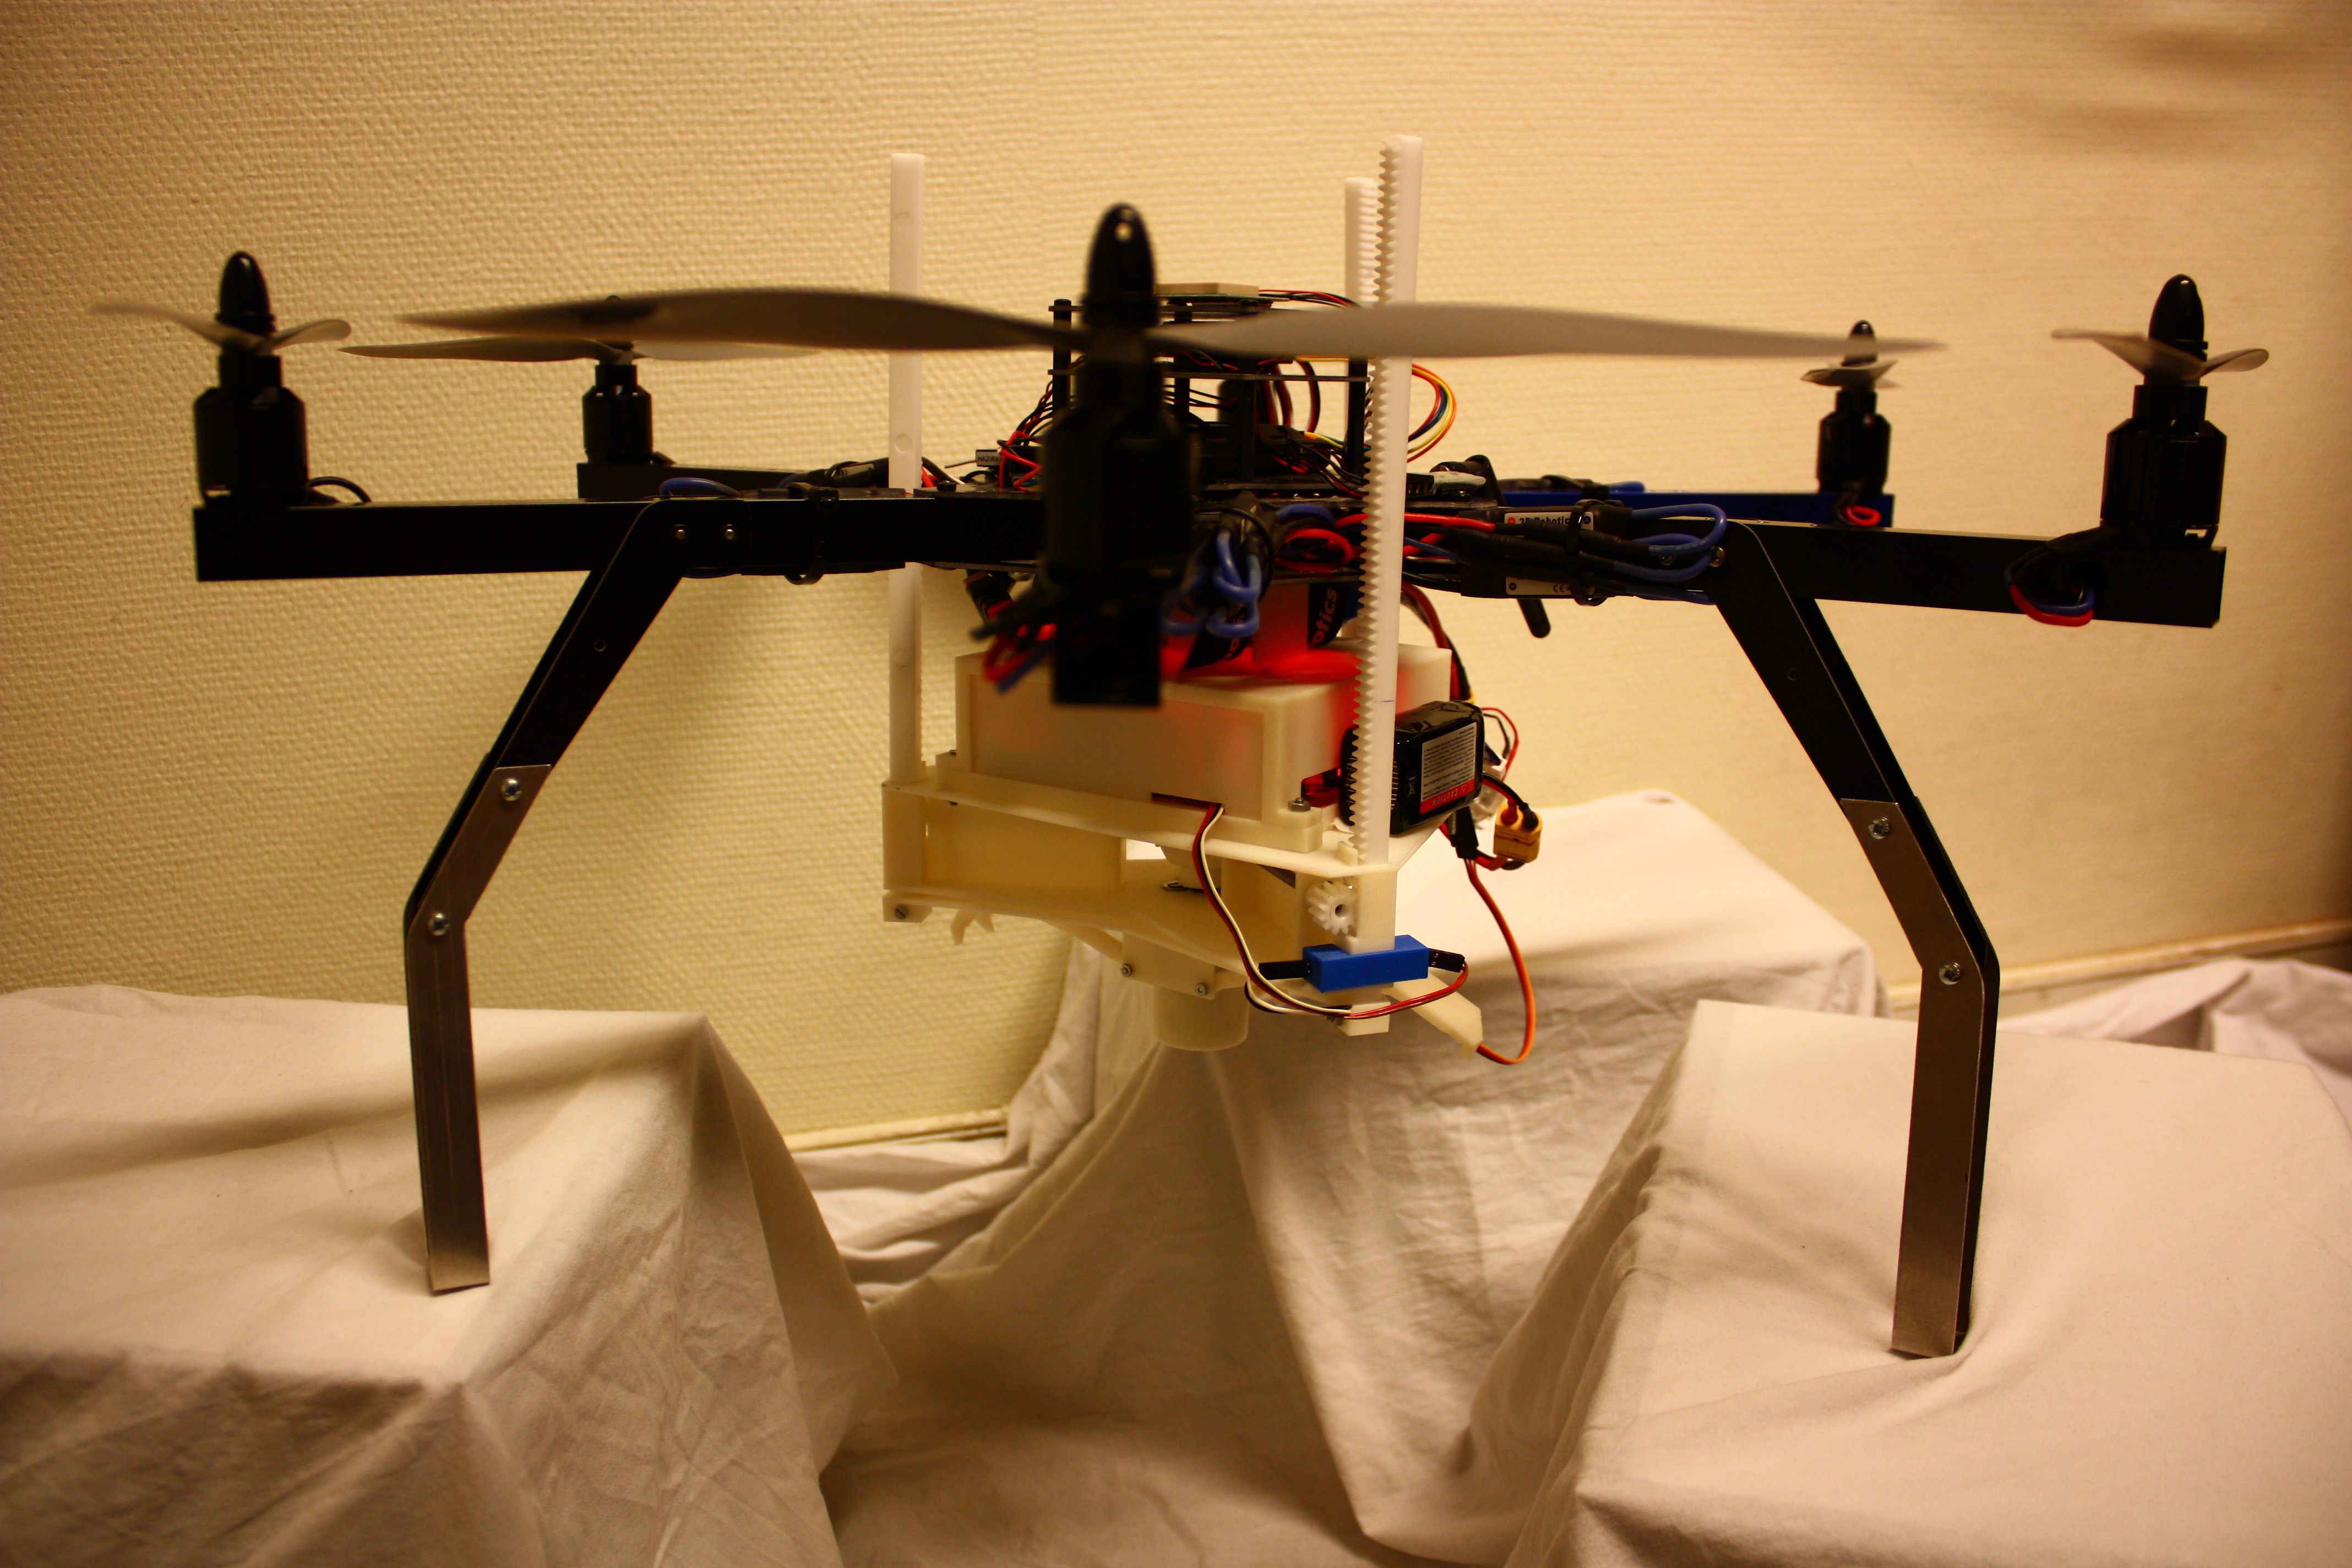
\includegraphics[width=7.95cm]{fig/finished/up.jpg}
\label{up}
}
\centering
\subfigure[Gripper lowered]{
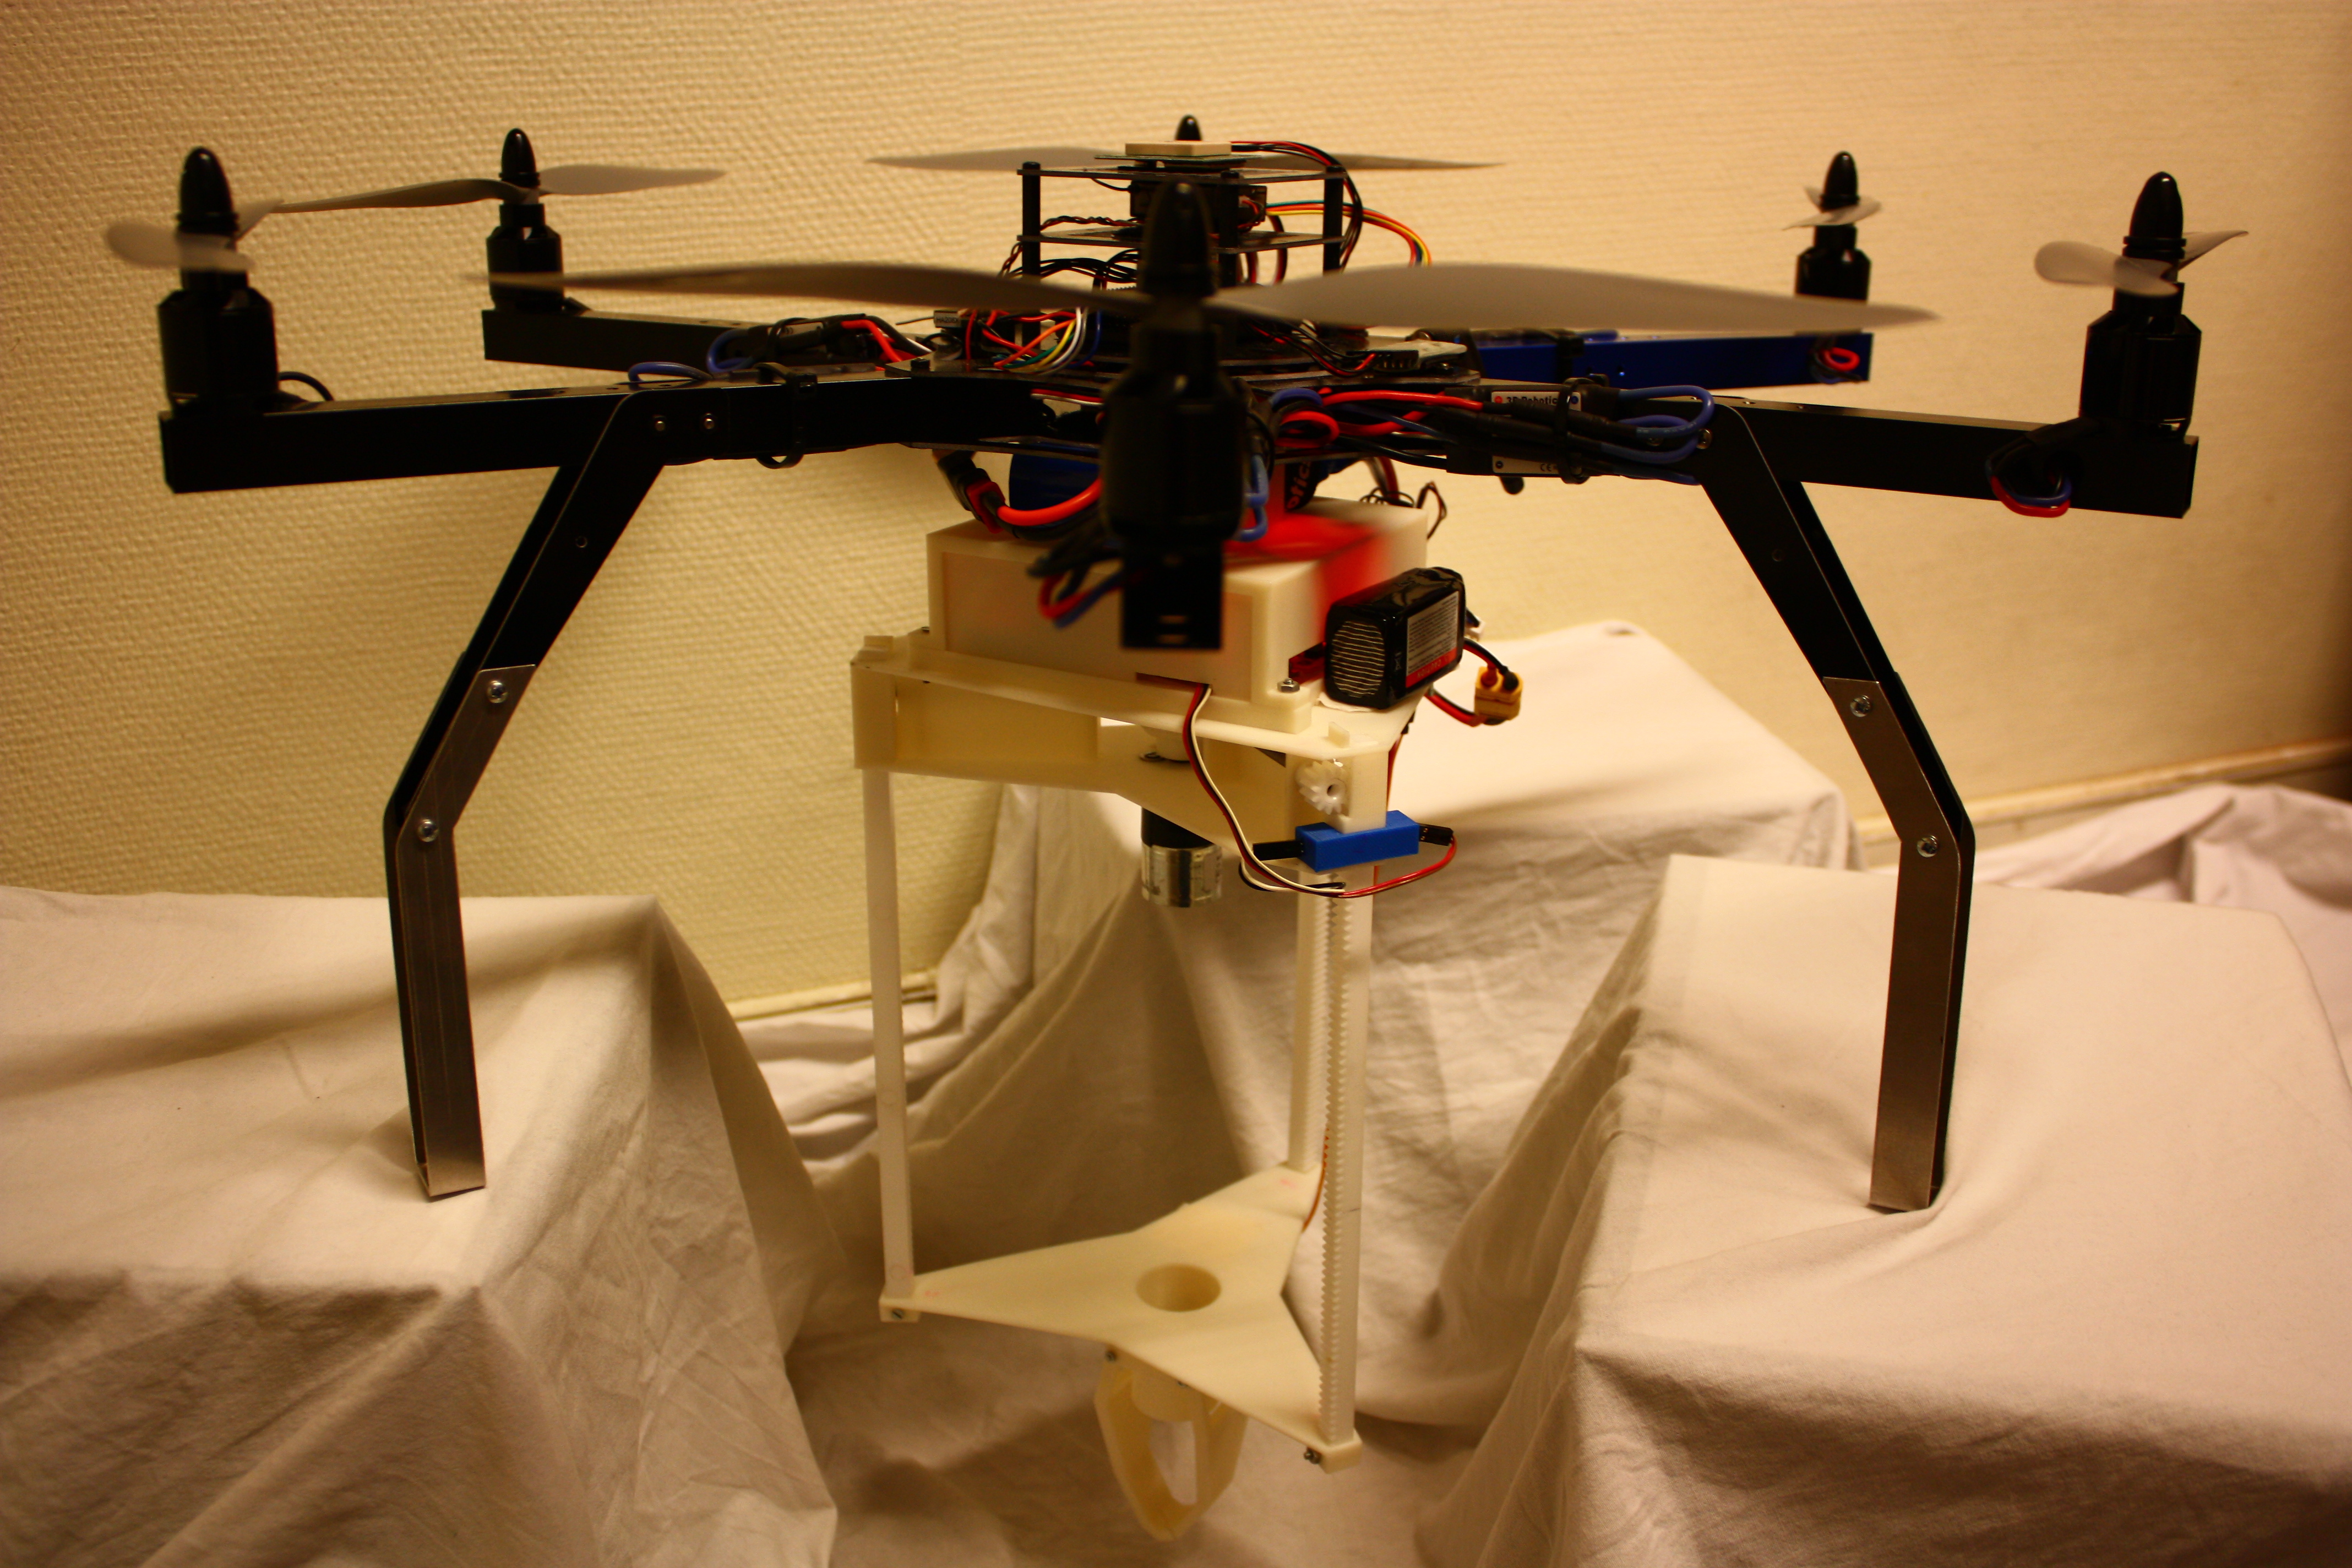
\includegraphics[width=7.95cm]{fig/finished/down.jpg}
\label{down}
}
\caption{Drop and recovery mechanism mounted to the hexacopter}
\label{finished}
\end{figure}
\section{Hardware}
\subsection{IR-LED Position Sensor}
The essence of the IR-LED position sensor is the IR-LED and the photodiode. These need some support circuitry to function. The circuit with the LED is fairly simple. It contains only of the IR-led and a resistor. The resistor is there to limit the current.\\\newline
The circuit for the photodiode is a bit more complicated. The photodiode chosen is a PIN type diode from Everlight. It is connected reversed biased, and does not conduct ordinarily, but starts to conduct when exposed to IR. The more IR the more it conducts. This last fact means that the signal will wary between 0 and 5 V depending on how much IR it ``sees". In this application the LED and the photodiode are mounted in a way that the photodiode only ``sees" the IR when the gripper platform is in position. Hence it is no need for an analog reading, the signal could be connected directly to a digital I/O port to give ether a in position or an out of position value. An opamp used as an voltage follower is included in the design, this isolates the output from the signal source. The operational amplifier used is an MC3405P from Motorola. A resistor is used to limit current.\\\newline
A decoupling capacitor was added. Decoupling capacitors are used to give noise a path to ground and keep the power in the circuit smooth \citep{embedded}. The schematics of the circuit design can be seen in Figure \ref{ledSchematic}. 
\begin{figure}[H]
\centering
\includegraphics[width = 15cm]{fig/krets/ledSchematic.jpg}
\caption{Schematics for the IR-LED Position Sensor}
\label{ledSchematic}
\end{figure}
\subsection{H-Bridge}
To be able to control direction and speed of the DC-motor lowering and raising the gripper, a H-bridge is needed. The H-bridge chosen for this is the DRV8801 h-bridge motor driver from Texas Instruments mounted to a break out board. The simplicity of this design makes it small in size and very low weight. Nominal output current is rated to 1 A, while it can handle peaks up to 2.8 A for a few seconds. It operates with motor supply voltages between 8 and 36 V and logic supply voltages between 3.3 and 6.5 volts \citep{h-bridge}. This makes it very versatile. The main drawback with the simplicity of this chip and break out board is that it could quite easily get over heated if driven with high current over time. This should not be a problem in this application because the nominal current of the chosen motor is given to be 50 mA and the time used to lower or raise the gripper is limited.
\subsection{Level Translator}
\label{level}
Communication will go both to and from the PandaBoard. The level translator will need at least eight channels, three for controlling the H-bridge, one for servo control, two for UART and two for the IR-LED position sensor signals. For this reason the  ADG3300BRUZ eight channel bidirectional level translator from Analog Devices was chosen. It is a convenient and easy to use level translator, just connect the desired low voltage and low voltage signals at one side and the desired hight voltage and high voltage signals at the other side. Two decoupling capacitors are also connected. The schematics of the circuit design can be seen in Figure \ref{levelTranslatorSchematic}.
\begin{figure}[H]
\centering
\includegraphics[width = 15cm]{fig/krets/levelTranslator.jpg}
\caption{Schematics for the Level Translator}
\label{levelTranslatorSchematic}
\end{figure}
\subsection{PWM-Controller}
The servo mounted to the gripper is controlled by using a PWM\footnote{Pulse Width Modulated}-signal. Where the time where the signal is high is transferable to the servos position reference. Typically is the time period for PWM signals controlling RC equipment 20 ms. With a high pulse of 1 ms meaning 0 degrees and 2 ms meaning 180 degrees. This means that to be able to control the servo in a stable and accurate way, the PWM-signal needs to be accurate. To get such an accurate signal using the PandaBoard can be challenging. It is possible to 
generate PWM with the PandaBoard using GPIO-pins and a real time operating system. But the operating system running on the PandaBoard in this project is a stripped down version of a Linux kernel without real time possibilities. In addition will the gripper be controlled through which further increases difficulties with timing.\\
\newline
To cope with this problems a PWM-controller was designed. The basis for the PWM-controller is an ATtiny85 8-bit microcontroller. This microcontroller is chosen for its simplicity. The microcontroller is programmed using ISP. To be able to program the microcontroller in circuit pins are added to all the pins, even though not all will be used in the application. This will also increase the possibilities for further developing if needed. A decoupling capacitor was also added to ensure noise free input voltage for the microcontroller.\\
\newline
Two bits will be used to control the PWM-controller with the PandaBoard. One bit turns on and off the signal, while the other bit gives the desired position of the gripper (either open or closed). The schematics of this circuit is shown in Figure \ref{pwm}, while the code running on the ATtiny85 is included in the digital appendix.
\begin{figure}[H]
\centering
\includegraphics[width = 16cm]{fig/krets/pwm.JPG}
\caption{Schematics for the PWM-Controller}
\label{pwm}
\end{figure}\noindent
\section{Communication Between the Modules}
An overview of the different modules and the communication between them is shown in Figure \ref{com}.\\
\newline
The PandaBoard communicates with the camera through a dedicated port that uses the MIPI CSI-2 standard. The rest of the communication to and from the PandaBoard goes via the level translator described in the previous section. The servo for the gripper is controlled with a PWM-signal while the H-bridge is controlled using three digital outputs. The communication between the PandaBoard and the APM uses UART and the MAVLink protocol. Relevant information here will be attitude and position data, and set points for the controller in the APM.
\begin{figure}[H]
\centering
\includegraphics[width = 12cm]{fig/krets/com.jpg}
\label{com}
\caption{Communication between the modules}
\end{figure}
\section{Power Supply}
The UAV contains a battery and a voltage regulator that regulates the voltage down to 5 V. It is possible to use this voltage source for the parts developed in this project. But using the regulated voltage source could easily result in to much current drawn, which will result in restarts of the APM and the Pandaboard. This could be disastrous for the UAV. To avoid this problem one could use a dedicated voltage regulator for the parts developed in this project, but that will decrease the range of the UAV and increase the chance of losing the UAV in case of problems with the parts developed in this project. Hence the safest and best solution is to add a separate battery and voltage regulator, this will increase weight which  will reduce range of the UAV, but this is considered to be a reasonable trade-off. To be able to decide which battery and voltage regulator to use, power demands are investigated and summarized in Table \ref{powerNeeds}.
\begin{table}[H]
\caption{Power demands}
\begin{center}
    \begin{tabular}{| l | l | l | l | l |}
    \hline
    \bf{Unit} & \bf{Voltage [V]} & \parbox{1.5cm}{\bf{Current} \bf{Peak [mA]}} & \parbox{1.5cm}{\bf{Current}\\ \bf{Normal [mA]}} & \bf{Source of info} \\ \hline
    Pandaboard & 5 & 1200 & 700\footnote{Based on tests of an earlier version of PandaBoard with CPU running at a 100 \% \cite{pandaboard_test}}& \parbox{4cm}{Pandaboard FAQ\\\citep{pandaboard}}\\ \hline
    Servo & 5 & 1500 & 800 & Measured\\ \hline
    DC motor & 12 & 50 & 50 &\parbox{4cm}{Data sheet \\\citep{motor}}\\ \hline
    Level Translator & 5 and 1.8 & 0.17E-3 & 5E-3 & \parbox{4cm}{Data sheet\\\citep{adg3300}}\\ \hline
    IR-LED Position Sensor & 5 & 150 & 450 & Measured\\ \hline
    Camera & 5 & 150 & 150 & \parbox{4.2cm}{Manufacturer web page\\\citep{camera_power}}\\\hline
    \bf{SUM} & - & \bf{3050} & \bf{2150} &\\\hline
    \end{tabular}
    \label{powerNeeds}
\end{center}
\end{table}\noindent
Selecting battery is a trade-off between capacity and weight. The battery should be able to power both the motor and the ICs\footnote{Integrated Circuits}. Hence a three cell Lithium-Polymer battery is chosen. These kind of batteries deliver 11.1 V, are able to deliver a lot of power fast and able to hold a lot of power in relation to its weight. The specific battery chosen is a 1000 mAh 20-30 C (means that it is able of delivering an instantaneous current of 20-30 times the capacity) battery from Haiyin. The battery is able to support the peak currents, but it might not be able to operate for very long if the servo and motor is used a lot in the mission. The battery will be replaced by a heavier one with greater capacity if necessary.\\
\newline
To reduce the chance for unstable voltages and current delivered to the PandaBoard, two voltage regulators are used, one for the PandaBoard and one for the rest of the equipment. Especially the servo can be a cause for ripple in the delivered voltage and current. This choices result in the power circuit displayed in Figure \ref{powerCircuit}.
\begin{figure}[H]
\centering
\includegraphics[width = 16cm]{fig/krets/power.jpg}
\caption{Power circuit}
\label{powerCircuit}
\end{figure}
\section{Camera Application}
The main application of the camera is to track the sensor node. The camera will also be used in the pickup to verify whether the gripper got hold of the sensor node or not (one could have used estimation of inertia for this task like \citep{Mellinger2011}, but the position of the camera makes it very convenient to use for this task). To be able to track the sensor node the camera will need to recognize the sensor node. This can be done in multiple ways as described briefly in Section \ref{opencv}. The SURF method can be efficient under the right circumstances, but some simple tests revealed some weaknesses. It turned out that only a few points on a picture of the pickup mount was marked as corners that it could use to search for. Of course the pickup mount could be made in a way that it would have more detail, but because it is quite small and it should be possible to detect at a distance this method was discarded. A classifier could be developed, but it will have weaknesses when it comes to rotation, and it would need a lot of example pictures to make it robust. Of this reasons the classifier solution was discarded as well. The much simpler solution of color detection was implemented.
\subsection{Tracking the Sensor Node}
\label{node}
To be able to use color detection the sensor node need to have some colors that sticks out. The mount for the sensor node (Figure \ref{sensorNode}) should have two different colors to make it possible to use color detection to get the orientation of the mount. The ocean is blue, which means that the sensor node should have colors that are as far away from blue on the HSV-wheel (Figure \ref{hsvWheel}). Yellow is an obvious choice because it is directly opposite of blue and it has a narrow band, which is good for noise cancellation. The colors next to yellow is red and green. Red contains both the lowest an highest hue values, which will make calculations more complex, hence green is chosen for the other color.\\
\newline
The picture from the camera is converted to the HSV-color space and copied to create two pictures. One of the pictures is thresholded with the HSV-values for yellow, while the other is thresholded with the values for green. This creates two binary pictures where the yellow and green fields are marked respectively. Then the "center of mass" of the two pictures are calculated. This centres of masses are used as centres of the two parts of the pickup mount and used to calculate the orientation of the mount and the center of the mount. This procedure is demonstrated in Figure \ref{color}. These points are in the picture frame. For the measurements to make sense one need a mapping from this pixel position to the position of the mount in NED.\\
\begin{figure}[H]
\centering
\subfigure[Original image]{
\includegraphics[width=7cm]{fig/colorRecognition/original.jpg}
}
\centering
\subfigure[HSV image]{
\includegraphics[width=7cm]{fig/colorRecognition/hsv.jpg}
}
\centering
\subfigure[Green thresholded]{
\includegraphics[width=7cm]{fig/colorRecognition/green.jpg}
}
\centering
\subfigure[Yellow thresholded]{
\includegraphics[width=7cm]{fig/colorRecognition/yellow.jpg}
}
\centering
\subfigure[Result]{
\includegraphics[width=7cm]{fig/colorRecognition/result.jpg}
}
\caption{Use of color recognition to track the mount of the sensor node}
\label{color}
\end{figure}\noindent
For control purposes a position of the sensor node in NED is good because this will be the same value as the error in position if the controller is trying to get to the exact position of the sensor node. For estimator and robustness the sensor nodes position should be referenced in ECEF. If the position of the sensor node is referenced in ECEF, it will be simpler to filter out weird measurements, estimation of the movements of the sensor node with current and waves becomes possible and the controller will have something to navigate towards even if the camera looses sight of the sensor node for a moment.\\\newline
To get the position of the sensor node in NED, first a transformation from BODY to NED is conducted by the use of the rotation matrix from BODY to NED in equation (\ref{R_ned}). DH convention is used to create consequential reference frames from BODY leading up to a reference frame in the sensor node. This is done to exploit the fact that the transformation matrix from BODY to the sensor node reference frame will contain the position of the sensor node reference frame expressed in BODY as seen in equation (\ref{T}).\\\newline
The first new frame is defined in the center of the camera lens. The homogeneous transformation $A_1$ from BODY to the camera frame is carried out as a movement $d_1$ along the BODY z-axis which gives the relation below. This coordinate frame and subsequent frames are visualized in Figure \ref{camera}. The parameters related to the transformations are also marked in the same figure.
\begin{eqnarray}
\boldsymbol{A}_1 = \begin{bmatrix}
1 & 0 & 0 & 0\\
0 & 1 & 0 & 0\\
0 & 0 & 1 & d_1\\
0 & 0 & 0 & 1
\end{bmatrix}
\end{eqnarray}
The next coordinate system is defined with the z-axis pointing towards the sensor node and the pixel position of the sensor node in the picture frame. This is done by rotating around the z-axis of $\alpha$ degrees and then rotating around the x-axis of $\beta$ degrees.\\\newline
To find $\alpha$ and $\beta$ some calculations needs to be done. The origin of the picture plane is in the topmost left corner. To get the angles to rotate, the origin is moved to the center of the picture frame by defining $\delta x = x_o - x_c$ and $\delta y = y_o - y_c$. The center of the picture frame is the point $(x_c, y_c)$ while the pixel position of the sensor node is the point $(x_o, y_o)$. The picture frame is defined to be at a distance of one meter away from the camera lens and the length between each pixel at this distance ($L$) is measured using an object of known length. The angles $\alpha$ and $\beta$ are then calculated.
\begin{eqnarray}
\alpha &=& atan2(\delta y, \delta x)\\
d &=& L\sqrt{\delta x^2 + \delta y^2}\\
\beta &=& \tan ^{-1}(d)\\
\end{eqnarray}
The resulting homogeneous transformation matrix is
\begin{eqnarray}
\boldsymbol{A}_2 = \begin{bmatrix}
c_\alpha & -s_\alpha & 0 & 0\\
s_\alpha & c_\alpha  & 0 & 0\\
0		 & 0		 & 1 & 0\\
0 		 & 0		 & 0 & 1
\end{bmatrix}
\begin{bmatrix}
1 & 0 		& 0 	   & 0\\
0 & c_\beta & -s_\beta & 0\\
0 & s_\beta & c_\beta  & 0\\
0 & 0		& 0		   & 1
\end{bmatrix}
= \begin{bmatrix}
c_\alpha	& -s_\alpha c_\beta		& s_\alpha s_\beta 		& 0\\
s_\alpha	& c_\alpha c_\beta	 	& -c_\alpha s_\beta 	& 0\\
0			& s_\beta			 	& c_\beta 				& 0\\
0			& 0						& 0						& 1
\end{bmatrix}
\end{eqnarray}
The last reference frame is defined in the sensor node. To get there a movement of $d_2$ along the z-axis is necessary. To calculate this distance, the angle ($\gamma$) between the z-axis in NED and the z-axis in the picture frame reference system needs to be calculated. The transformation matrix from NED to picture frame is calculated to be able to read out the direction of the z-axis in the picture frame reference system.
\begin{eqnarray}
\boldsymbol{T}_{pf}^{n} = \boldsymbol{R}_b^n(\boldsymbol{\Theta} _{nb})\boldsymbol{A}_1\boldsymbol{A}_2
\end{eqnarray}
Out of this transformation matrix one can read out the direction of the z-axis of the picture frame reference system $\boldsymbol{z} _{pf}^n$ while the direction of the z-axis of NED is trivial.
\begin{eqnarray}
\boldsymbol{z}_{pf}^n = \begin{bmatrix}
s_\alpha s_\beta c_\psi c_\theta - c_\alpha s_\beta (-s_\psi c_\phi + c_\psi s_\theta s_\phi) + c_\beta (c_\psi c_\phi + s_\psi s_\theta s_\phi)\\
s_\alpha s_\beta s_\psi c_\theta -c_\alpha s_\beta (c_\psi c_\phi + s_\psi s_\theta s_\phi) + c_\beta (-c_\psi s_\phi + s_\psi s_\theta s_\phi)\\
-s_\alpha s_\beta s_\theta - c_\alpha s_\beta c_\theta s_\phi + c_\beta c_\theta c_\phi
\end{bmatrix}
	\boldsymbol{z}_n^n = \begin{bmatrix}
	0\\0\\1
	\end{bmatrix}
\end{eqnarray}
The angle $\gamma$ between these two vectors can be calculated using dot product, and the fact that the vectors in the rotation matrices are normalized. This combined with basic trigonometry gives these two relations.
\begin{eqnarray}
\cos \gamma &=& \dfrac{\boldsymbol{z}_{pf}^n\cdot \boldsymbol{z}_n^n}{|\boldsymbol{z}_{pf}^n||\boldsymbol{z}_n^n|} = z_{pf_3}^n\\
\cos\gamma &=& \dfrac{h - d_1c_\theta c_\phi}{d_2}
\end{eqnarray}
These relations combined gives the following expression for $d_2$ and the homogeneous transform.
\begin{eqnarray}
d_2 &=& \dfrac{h - d_1c_\theta c_\phi}{z_{pf_3}^n}\\
\boldsymbol{A}_3 &=& \begin{bmatrix}
1 & 0 & 0 & 0\\
0 & 1 & 0 & 0\\
0 & 0 & 1 & d_2\\
0 & 0 & 0 & 1
\end{bmatrix}\\
\boldsymbol{T}_{obj}^n &=& \boldsymbol{T}_{pf}^{n}\boldsymbol{A}_3
\label{T_last}
\end{eqnarray}
Calculations of equation (\ref{T_last}) will read out the position of the origin of the reference frame in the sensor node (according to equation (\ref{T})). This gives
\begin{eqnarray}
\boldsymbol{p}_{obj}^n = \begin{bmatrix}
d_2z_{pf_1}^n + d_1(s_\psi s_\phi + c_ \psi s_\theta c_\phi)\\
d_2z_{pf_2}^n + d_1(-c_\psi s_\phi + s_\psi s_\theta c_\phi)\\
h
\end{bmatrix}
\end{eqnarray}
For the purpose of tracking this vector is then transformed into the ECEF coordinate frame by the transform in equation (\ref{ecef}).
\begin{figure}[H]
\centering
\includegraphics[width = 18cm]{fig/camera.jpg}
\caption{Visualization of the different coordinate systems}
\label{camera}
\end{figure}

\chapter{Control Software}
\label{control_SW}
\begin{figure}[H]
\centering
\includegraphics[width = 12cm]{fig/SW.jpg}
\caption{Software structure}
\label{SW}
\end{figure}
\chapter{Simulation of the System}
To be able to verify the controller and the general control structure, the system was simulated using MATLAB and Simulink. This meant that a mathematical model of the hexacopter needed to be derived and that the low level controllers and thrust allocation of the APM needed to be simulated using some approximations and assumtions on its behaviour. The different models are derived below, then they are put together to a full system including the controller to be able to put the controller to the test.
\section{Mathematical Model of the Hexacopter}
\begin{figure}[H]
\centering
\includegraphics[width = 8cm]{fig/model.jpg}
\caption{Model of hexacopter \textit{Courtesy of \citep{model}}}
\label{model}
\end{figure}
To model the dynamics of the hexacopter equations (\ref{RB}) and (\ref{RB2}) are used. The key component that needs to be derived is the torque vector $\boldsymbol{\tau}_{RB}$, which is expressed in the BODY-frame. The thrust from each propeller is according to \citep{model} expressed as a lift constant times the squared angular speed of the propeller. In addition they approximate the moment caused around the propeller axis as a drag constant times the squared angular speed of the propeller plus the inertia moment of the propeller times the angular acceleration of the propeller. This is shown in equations (\ref{model2}) and (\ref{model3}).
\begin{eqnarray}
\boldsymbol{f}_i = \begin{bmatrix}
0 & 0 & k\omega_i^2
\label{model2}
\end{bmatrix}^T\\
\tau_{M_i} = b\omega_i^2 + I_{M_i}\dot{\omega}_i
\label{model3}
\end{eqnarray} 
Where $k$ is the lift constant, $b$ is the drag constant, $I_m$ is the inertia moment of a propeller and $\omega_i$ is the angular speed of propeller $i$. These equations and some simple geometry gives the following force and moment balances, where $\phi$ is the roll angle, $\theta$ is the pitch angle and $l$ is the length of the arm from the center of gravity to the center of the propeller.
\begin{eqnarray}
\boldsymbol{\tau}_{RB} = \begin{bmatrix}
-mg\sin(\theta)\\
mg\cos(\theta)\sin(\phi)\\
mg\cos(\theta)\cos(\phi) - k \sum_{i=1}^6\omega_i^2\\
kl(-\dfrac{1}{2}\omega_1^2 +\dfrac{1}{2}\omega_2^2 + \omega_3^2 +\dfrac{1}{2}\omega_4^2 -\dfrac{1}{2}\omega_5^2 -\omega_6^2\\
\dfrac{\sqrt{3}}{2}kl(\omega_1^2 + \omega_2^2 - \omega_4^2 - \omega_5^2)\\
b(\omega_1^2 - \omega_2^2 + \omega_3^2 - \omega_4^2 + \omega_5^2 - \omega_6^2) + I_m(\dot{\omega}_1^2 + \dot{\omega}_2^2 + \dot{\omega}_3^2 + \dot{\omega}_4^2 + \dot{\omega}_5^2 + \dot{\omega}_6^2)
\end{bmatrix}
\label{tau}
\end{eqnarray}
Not considering the different parameters, all the information needed to use equations (\ref{RB}) and (\ref{RB2}) are present, which gives.
\begin{eqnarray}
\dot{\boldsymbol{\nu}} = \boldsymbol{M}_{RB}^{-1}(\boldsymbol{\tau}_{RB} - \boldsymbol{C}_{RB}(\boldsymbol{\nu})\boldsymbol{\nu})
\end{eqnarray}
This equation is then transformed to the NED frame using the rotation matrix in equation (\ref{R_ned}) and the transformation matrix in equation (\ref{trans}) as shown in equation (\ref{eta}).
\begin{eqnarray}
\boldsymbol{\eta} = \begin{bmatrix}
\boldsymbol{R}_b^n(\boldsymbol{\Theta}_{nb}) & \boldsymbol{0}_{3 \times 3}\\
\boldsymbol{0}_{3 \times 3} & \boldsymbol{T}_\Theta(\boldsymbol{\Theta}_{nb})
\end{bmatrix}
\boldsymbol{\nu}
\label{eta}
\end{eqnarray}
Where $\boldsymbol{\eta} = [\boldsymbol{p}^n, \boldsymbol{\Theta}_{nb}]^T$ is the position in NED and the Euler angles.
\section{Simulation of Low Level Controllers and Thrust Allocation in the APM}
The attitude controllers in the APM are approximated as PD-controllers. One must assume that the controllers of the APM follows the references given, PD-controllers will do this, hence this is a fair approximation. The height controller of the APM is approximated as a PID-controller.\\
\newline
%The purpose of the thrust allocation algorithm is to convert desired force or moments in the different degrees of freedom into desired thrust from the different motors. A way to manage this is proposed and derived in \citep{sorensen} is rendered here.\\
%\newline
%The relationship between the control vector
The purpose of the thrust allocation algorithm is to convert desired force or moments in the different degrees of freedom into desired thrust from the different motors. The control vector given by the height and attitude controllers will contain desired thrust in negative z-direction and desired moments around the different axes. This vector is given by $\boldsymbol{\tau}_c = [T\; \tau_{\phi_c}\; \tau_{\theta_c}\; \tau_{\psi_c}]^T$. Using equation (\ref{tau}) combined with the control vector gives the following relationship.
\begin{eqnarray}
\boldsymbol{\tau}_{c} &=& \begin{bmatrix}
k & k & k & k & k & k\\
-\dfrac{1}{2}kl & \dfrac{1}{2}kl & kl & \dfrac{1}{2}kl & -\dfrac{1}{2}kl & -kl\\
\dfrac{\sqrt{3}}{2}kl & \dfrac{\sqrt{3}}{2}kl & 0 & -\dfrac{\sqrt{3}}{2}kl & -\dfrac{\sqrt{3}}{2}kl & 0\\
b & -b & b & -b & b & -b
\end{bmatrix}
\begin{bmatrix}
\omega_1^2\\
\omega_2^2\\
\omega_3^2\\
\omega_4^2\\
\omega_5^2\\
\omega_6^2
\end{bmatrix}
= \boldsymbol{A}\boldsymbol{u}\\
\boldsymbol{u} &=& \boldsymbol{A}^+\boldsymbol{\tau}_c \label{u_motor}\\
\boldsymbol{A}^+ &=& \boldsymbol{A}^T(\boldsymbol{A}\boldsymbol{A}^T)^{-1}\label{pseudo}
\end{eqnarray}
The desired input to each motor is calculated using equation (\ref{u_motor}), where the pseudo inverse of $\boldsymbol{A}$ is calculated as shown in equation (\ref{pseudo}).
\section{Simulation of the Camera Algorithm}
To simulate the measurements from the camera, the algorithm given in Section \ref{node} is used to find the position of each of the corners of the camera frame. Then a ray casting algorithm is used to determine if the position of the sensor node is within the camera frame. The ray casting algorithm is outside the scope of this report.\\
\newline
If the sensor node is within the camera frame, perfect measurements of both node position in relation to the hexacopter and the heading of the node are sent back to the control algorithm.
\section{Simulink Model}
All the components for the simulator explained abov,e in addition to a PandaBoard component containing the controller described in the previous chapter is put together to create the Simulink model shown in Figure  \ref{simulink}.
\begin{figure}[H]
\centering
\includegraphics[width = 18cm]{fig/simulink.jpg}
\caption{Simulink}
\label{simulink}
\end{figure}
\section{Test of Controller}
The main scenario simulated is as close to the lab tests that will be conducted as possible. As the main challenge of the hexacopter controller is the pickup phase, the simulation will focus on this phase. In each of the simulations the hexacopter ramps up from a ground start to a height of 4 m. The sensor node is assumed to be lying 0.5 m North and 0.5 m East of the starting point. As the  hexacopter is flying the simulated camera will give measurements of the position of the sensor node, but only if the sensor node would have been in the camera frame. If the camera is unable to spot the sensor node, the position reference used for the controller will be the current position. The hexacopter will also try to maintain the same heading as the sensor node. If the sensor node is in the camera frame, the reference heading for the hexacopter will be updated, if the view of the sensor node is lost, the reference will be the last measured node heading\\
\newline
Three scenarios will be simulated, first a simulation with no disturbances, then a simulation with constant disturbance and lastly a simulation with varying disturbances.
\subsection{Simulation Without Disturbances}
The scenario was first simulated using the proposed controller from equation (\ref{u}) without any disturbances present.
\subsubsection{Results}
The North-East-Down position of the sensor node is plotted in Figure \ref{posNoDisturbance}. It can be seen from the figure how the reference position is updated when the camera spots the sensor node. And one should also note that the hexacopter ramps down all the way to the sensor node without loosing sight of the sensor node. 
\begin{figure}[H]
\centering
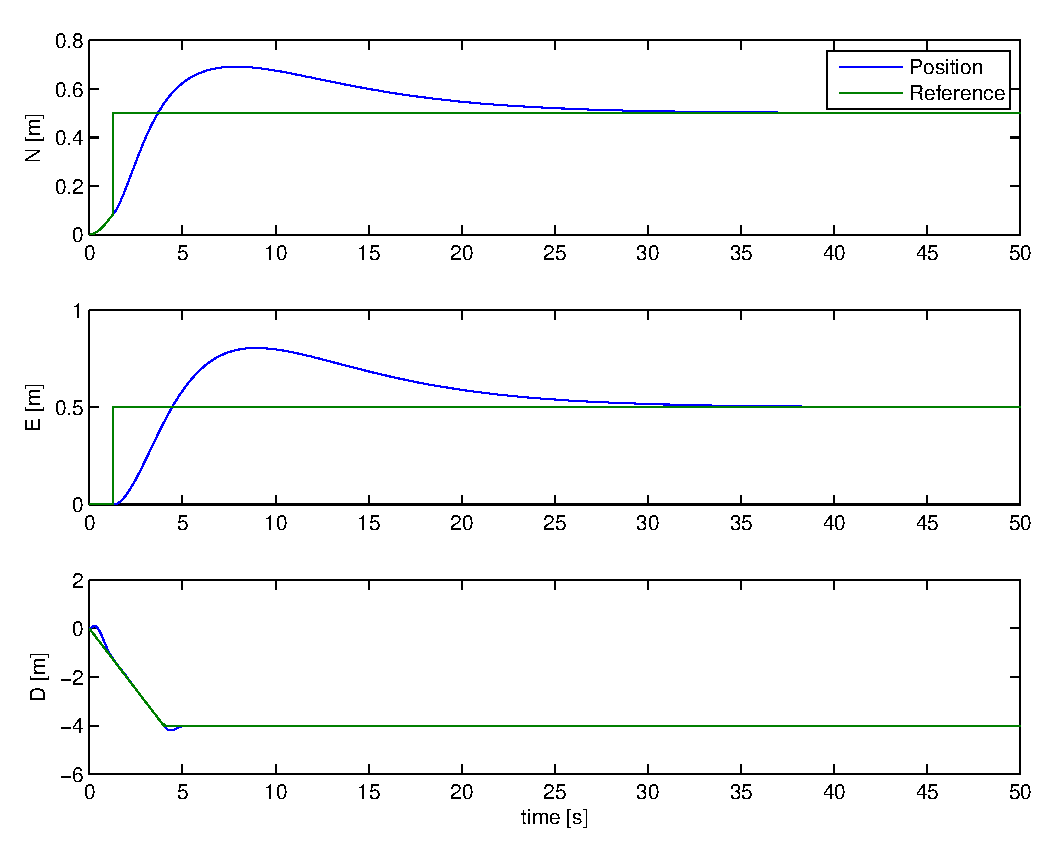
\includegraphics[width = 12cm]{fig/plots/simulation/positionNoDisturbance.eps}
\caption{North-East-Down position of the hexacopter}
\label{posNoDisturbance}
\end{figure}
\noindent
Figure \ref{posFrameNoDisturbance} shows the the North-East position of the hexacopter and the sensor node. It also shows the camera frame and whether the node is spotted by the camera or not. It can also be seen from this plot how the hexacopter yaws to keep the same heading as the sensor node (this can be seen even better from attitude plots shown in  Appendix A). 
\begin{figure}[H]
\centering
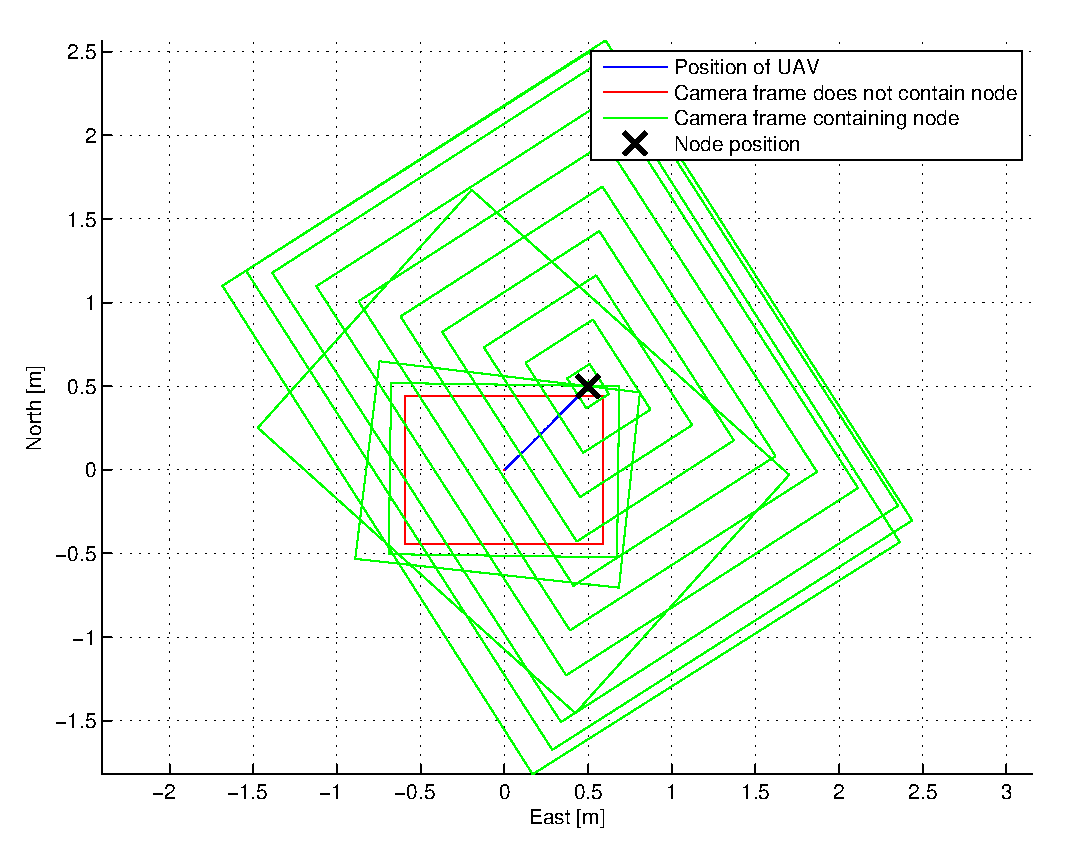
\includegraphics[width = 12cm]{fig/plots/simulation/positionFrameNoDisturbance.eps}
\caption{North-East-Down position of the hexacopter, sensor node and camera frame}
\label{posFrameNoDisturbance}
\end{figure}
\subsubsection{Discussion}
The hexacopter is able to lower itself down on the exact spot of the sensor node without loosing sight of the sensor node. This is very promising results, although some early tests in the lab showed that the controller used in this simulation would give some stationary deviations. The lab tests were conducted inside so wind played no part in this error. The error is probably due to unbalances of the hexacopter and inaccuracies of the low level controllers of the APM. Hence integral action was added to the controller. A simulation with constant disturbance and integral action follows.
\subsection{Simulation With Constant Disturbances}
The disturbance added could for instance represent a wind affecting the hexacopter with a force of 0.5 N in North-direction.
\subsubsection{Results}
As can be seen from Figure \ref{posFrameDisturbance} and Figure \ref{posFrameDisturbance} the hexacopter overshoots the reference position. The controller is able to cancel out the disturbance and make the hexacopter descend upon the sensor node.
\begin{figure}[H]
\centering
\includegraphics[width = 12cm]{fig/plots/simulation/positionDisturbance.eps}
\caption{North-East-Down position of the hexacopter}
\label{posDisturbance}
\end{figure}
\begin{figure}[H]
\centering
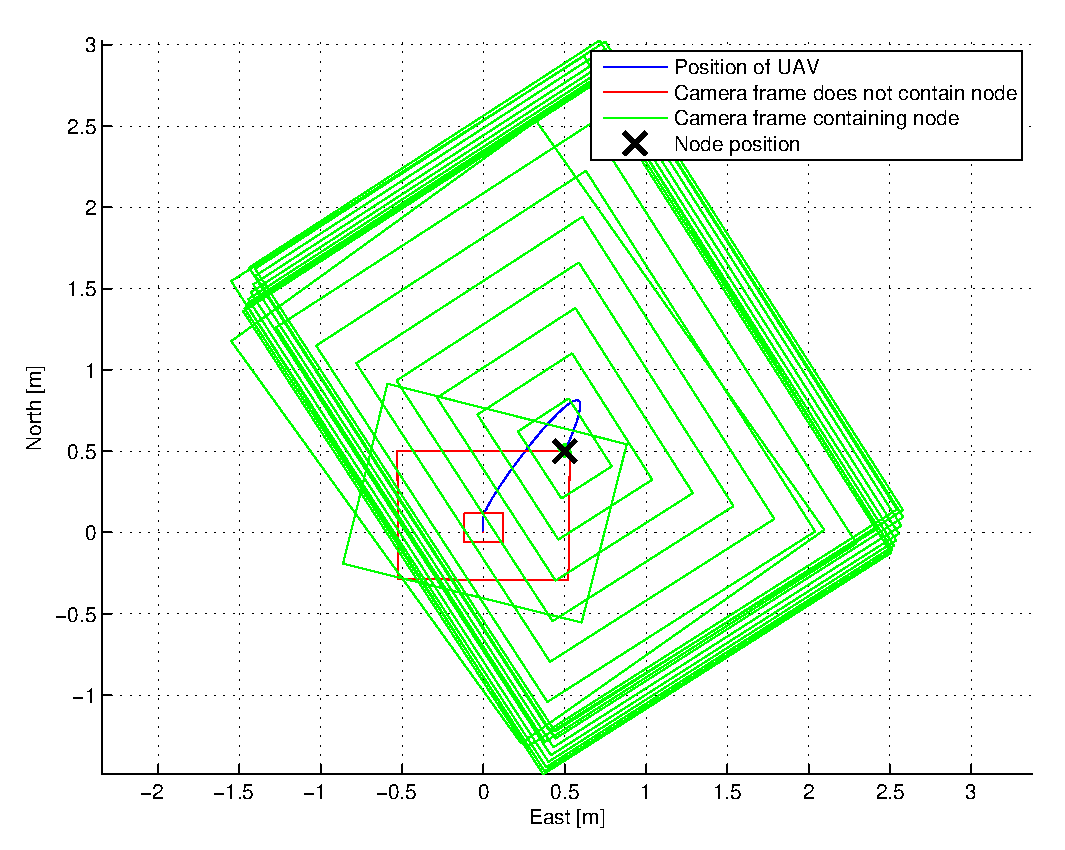
\includegraphics[width = 12cm]{fig/plots/simulation/positionFrameDisturbance.eps}
\caption{North-East-Down position of the hexacopter, sensor node and camera frame}
\label{posFrameDisturbance}
\end{figure}
\subsubsection{Discussion}
The overshoot of the position reference is due to the I-term of the controller and is quite natural due to the step in reference position. The fact that the disturbances is working in North-direction will also lead to an overshoot in North-direction, due to the added forces in that direction. The controller is able to correct for the disturbance and descend upon the sensor node, which is very good. 
\subsection{Simulation With Varying Disturbances}
The controller is tested in simulations where the disturbances are varying in both North and East-direction using integrated band limited white noise where the integral is limited by $\pm$ 1 N in both directions. The magnitude and direction of the disturbance is plotted in the appendix.
\subsubsection{Results}
The hexacopter stays approximately straight above the sensor node, and is able to lower itself a bit down towards the sensor node before it looses the sight of the node and drifts away. Both these observations are easily seen in Figures \ref{posVarDisturbance} and \ref{posFrameVarDisturbance}.
\begin{figure}[H]
\centering
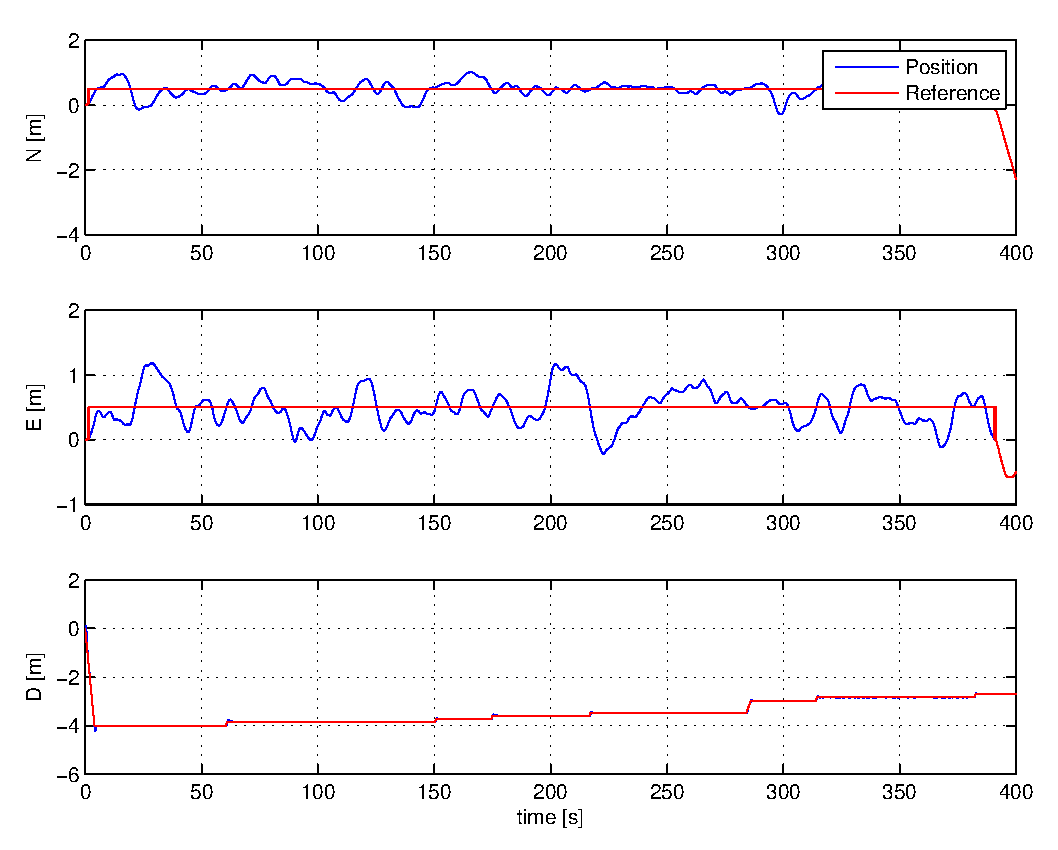
\includegraphics[width = 12cm]{fig/plots/simulation/positionVarDisturbance.eps}
\caption{North-East-Down position of the hexacopter}
\label{posVarDisturbance}
\end{figure}
\begin{figure}[H]
\centering
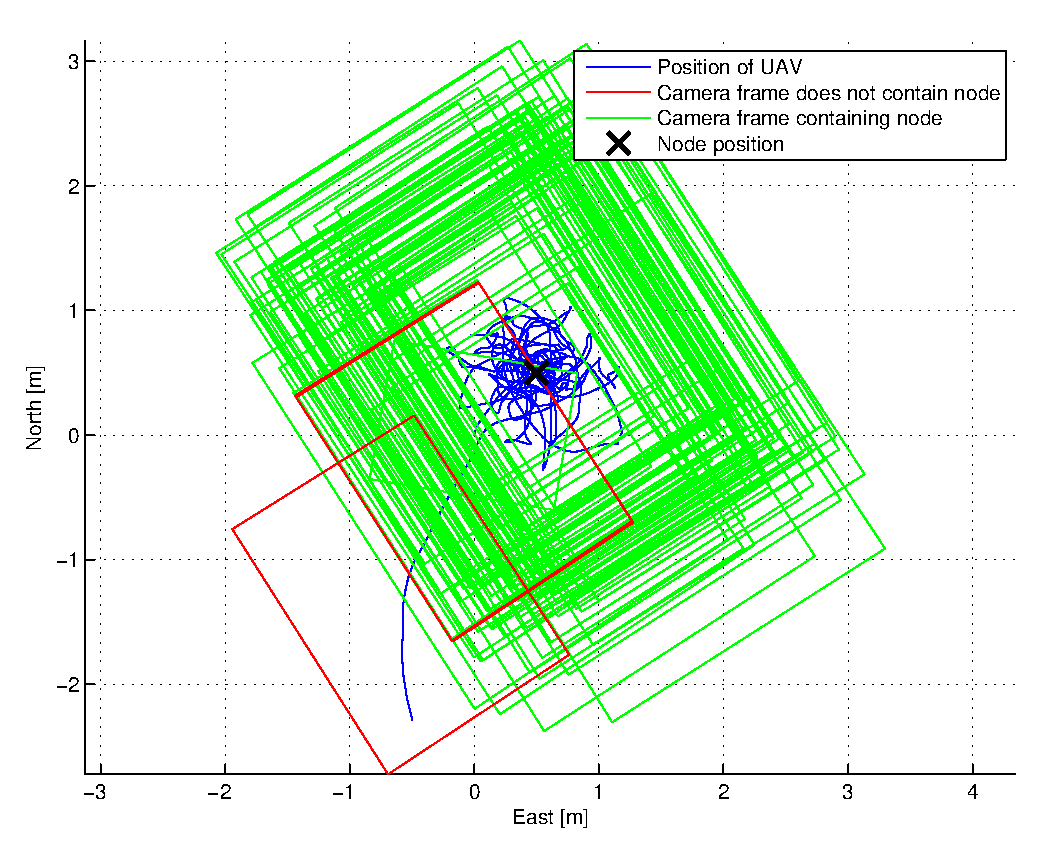
\includegraphics[width = 12cm]{fig/plots/simulation/positionFrameVarDisturbance.eps}
\caption{North-East-Down position of the hexacopter, sensor node and camera frame}
\label{posFrameVarDisturbance}
\end{figure}
\subsubsection{Discussion}
The results show that the controller is able to handle some random disturbances but sooner or later these disturbances will lead to problems where the camera will loose sight of the sensor node and then drift off. This will make pick up in such conditions impossible.
\subsection{Simulation With Constant Disturbances on the Hexacopter and Disturbances Affecting the Sensor Node}
A more realistic simulation is to simulate the system with constant disturbance, e.g. due to wind or inaccuracies in the APM. And let the sensor node be affected by some varying noise, which makes it change heading and position. The noise is modelled as random walk.
\subsubsection{Results}
As seen from Figures \ref{posNodeDisturbance} and \ref{posFrameNodeDisturbance} the hexacopter tracks both position and heading of the sensor node, and is actually able to get down to 5 cm above the sensor node before loosing sight of it and drifting off.
\begin{figure}[H]
\centering
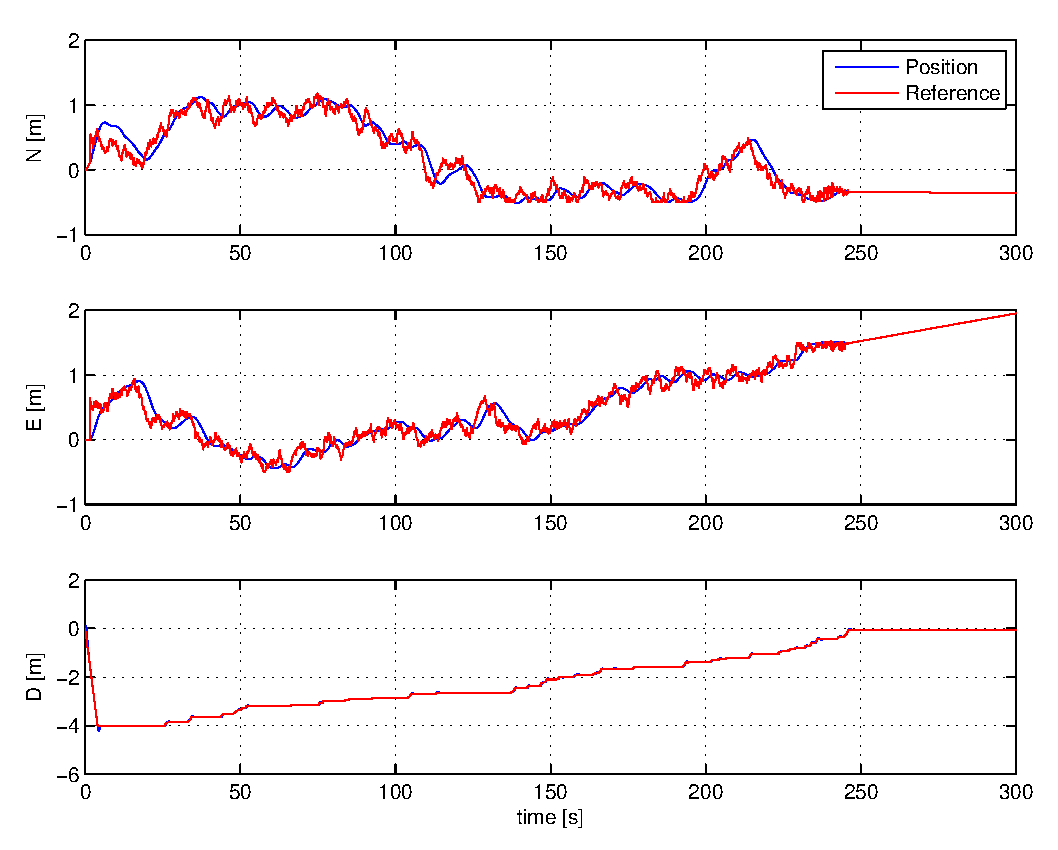
\includegraphics[width = 12cm]{fig/plots/simulation/positionNodeDisturbance.eps}
\caption{North-East-Down position of the hexacopter}
\label{posNodeDisturbance}
\end{figure}
\begin{figure}[H]
\centering
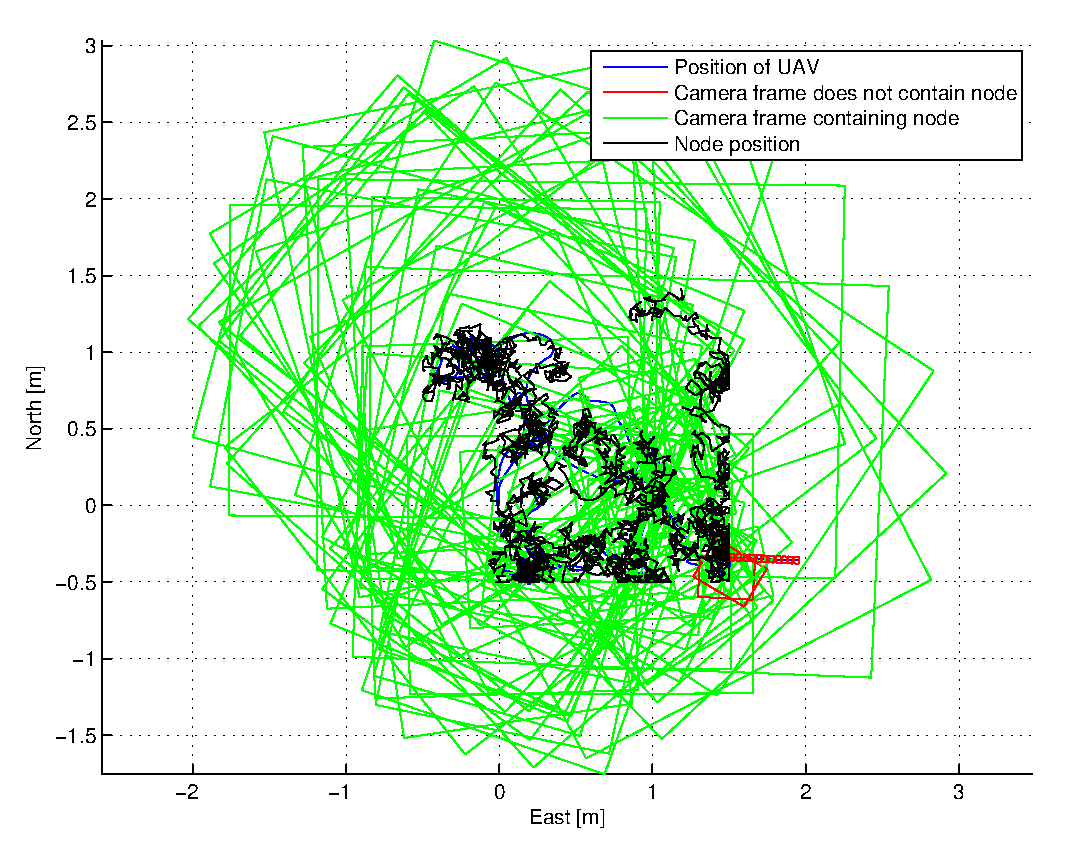
\includegraphics[width = 12cm]{fig/plots/simulation/positionFrameNodeDisturbance.eps}
\caption{North-East-Down position of the hexacopter, sensor node and camera frame} 
\label{posFrameNodeDisturbance}
\end{figure}
\subsubsection{Discussion}
The hexacopters abilities to track the sensor nodes position and heading is quite promising. The main issue that is revealed is the need for some way to get back to the previous position where the sensor node was spotted last. The simulations have also shown that this setup is not able to handle rough weather conditions, meaning that operation should be limited to days with only small waves and little wind.
\chapter{Testing and Results}
\section{Node Tracking}
Points for node tracking test:
- Equipment
	- Panda or Computer; Panda, computer for Neptus
	- Implementere sonar igjen
	- Sende bilder til Neptus / Dune
	- laser
	- kompass
\subsection{Result of Test}
\include{chapter07}
\include{chapter08}
% Include more chapters as required.
%%=========================================
%\appendix
	% Include more appendices as required.
%%=========================================
\bibliographystyle{apa}
\addcontentsline{toc}{chapter}{\bibname}
\bibliography{bibtex/scopus}  
\end{document}